%---------------------导言区---------------------------%
\documentclass[12pt,a4paper,UTF8]{ctexart}
	%10pt：正文字体为12pt，缺省为10pt；各层级字体大小会根据正文字体自动调整
	%a4paper：纸张大小a4；
	%UTF8：中文要求
\usepackage{geometry}%用于设置上下左右页边距
	\geometry{left=2.5cm,right=2.5cm,top=3.2cm,bottom=2.8cm}
\usepackage{xeCJK}
\usepackage{amsmath}
\usepackage{paralist}
\usepackage{enumerate}
\usepackage{booktabs}
\usepackage{multirow}
\usepackage{graphicx}
\usepackage{subfig}
\usepackage{setspace}
\usepackage{listings}
\usepackage{lastpage}
\usepackage{hyperref}
\usepackage{pdfpages}

%xeCJK：中文字体（如楷体，作者和机构需要用到）的设置
	%amsmath：数学公式
	%paralist，enumerate：自定义项目符号
	%booktabs：三线图，论文常用的表格风格
	%multirow：复杂表格
	%graphicx，float: 插入图片
	%subfig：并排排版图片、竖向排版图片
	%setspace：设置行间距等功能
	\setlength{\parindent}{2em}%正文首行缩进两个汉字
	%listings:用于排版各种代码；比如matlab的代码
	\lstset{language=Matlab}%matlab代码
	%lastpage:获取总页数;
	%hyperref:超链接,和lastpage搭配.
\usepackage{fancyhdr}
	%fancyhdr：一个很强大的宏包，用于自定义设计页面风格并命名以供调用。
	\pagestyle{fancy}
	\rhead{塞曼效应实验}
	\lhead{近代物理实验~~~实验报告}
	\cfoot{Page \thepage/\pageref{LastPage}}  %当前页\总页数
	\rfoot{\today}
		%分别是右页眉、左页眉、中页脚、右页脚
	\renewcommand{\headrulewidth}{0.4pt}
	\renewcommand{\theenumi}{(\arabic{enumi})}

%%%%%%%%%%%%%%%%%%%%%%%%%%%%%%%%%%%%%%%%%%%%%%%%%%%%%%%%%%
%%%%%%%%%%%%%%%%%%%%%%%%%正文开始%%%%%%%%%%%%%%%%%%%%%%%%%%
%%%%%%%%%%%%%%%%%%%%%%%%%%%%%%%%%%%%%%%%%%%%%%%%%%%%%%%%%%

\graphicspath{{wzc_xsx_Zeeman/}{wzc_xsx_Zeeman_week2/}}
\begin{document}

%%begin-------------------标题与信息-----------------------%%

%%标题
\begin{center}
\LARGE\textbf{塞曼效应实验}
\end{center}

%%信息
\begin{doublespacing}
	%doublespacing：手动两倍行距
	\begin{tabular}{lr}
	 & \\
	 {实验人姓名：徐殊行~23343071} & {合作者姓名：王志超~23343062}\\
	 {实验时间：2025年5月30日/6月4日} & {室温：29$^{\circ}$C~相对湿度：65\%}
	
	\end{tabular}
\end{doublespacing}

%%-------------------中英文摘要-----------------------%%
\begin{abstract}
  \noindent 塞曼效应实验旨在通过观测原子光谱在外加磁场下的分裂现象，验证原子磁矩与空间量子化，并测定电子荷质比 $e/m$、能级的量子数 $J$、磁量子数 $M$ 及郎德因子 $g$。
  实验采用笔型汞灯发射光源，通过电磁铁产生可调磁场，使用法布里–珀罗（Fabry–Pérot）标准具记录干涉花样。
  基于多光束干涉原理，测量在不同磁场强度下干涉环直径的微小变化，计算谱线的波长裂分，进而反推出电子的基本参数和原子能级信息。
  实验还利用偏振片区分 $\pi$ 线与 $\sigma^\pm$ 线，并研究横向与纵向观察条件下的谱线偏振特性。
  本实验不仅巩固了塞曼效应的理论基础，还培养了法布里–珀罗干涉测量技术和 CCD 图像处理能力，为进一步探究原子内部结构提供了实验手段。\cite{zhu1979atom,wu1978optics,xu1993modernphysics}

    \noindent \textbf{关键词：} 塞曼效应；法布里–珀罗标准具；荷质比；朗德因子；原子能级分裂；干涉测量；CCD 图像处理
		
\end{abstract}
	
\renewcommand{\abstractname}{Abstract}

\begin{abstract}
  \noindent The Zeeman effect experiment aims to observe the splitting of atomic spectral lines under an external magnetic field, thereby verifying atomic magnetic moments and spatial quantization, 
  as well as determining the electron charge-to-mass ratio ($e/m$), energy-level quantum numbers ($J$, $M$), and the Landé $g$-factor. 
  A pen-type mercury lamp serves as the light source, while an adjustable electromagnet provides a known magnetic field. 
  A Fabry–Pérot interferometer captures high-resolution interference patterns. By recording the subtle changes in the diameters of interference fringes at various magnetic field strengths, 
  the experiment calculates the wavelength shifts of Zeeman-split lines and derives fundamental parameters such as $e/m$ and $g$. 
  Polarizers distinguish between $\pi$ and $\sigma^\pm$ components, enabling the study of spectral polarization in both transverse and longitudinal observation geometries. 
  The procedure integrates Fabry–Pérot interferometry, CCD-based image acquisition, and data analysis to compare measured results with theoretical predictions. 
  This experiment reinforces the theoretical foundation of the Zeeman effect and develops practical skills in high-resolution spectroscopy and image processing, 
  offering a robust approach to probing atomic internal structure.
    
	\noindent \textbf{Keywords: } Zeeman Effect; Fabry–Pérot Interferometer; Charge-to-Mass Ratio; Landé g-Factor; Atomic Level Splitting; Interference Measurement; CCD Image Processing
\end{abstract}

%%-------------------正文部分-----------------------%%

\subsection*{【实验目的】}
\begin{enumerate}[(1)]
    \item 掌握塞曼效应理论，测定电子的荷质比，确定能级的量子数和朗德因子，绘出跃迁的能级图；
    \item 掌握法布里－珀罗标准具的原理和使用；
    \item 观察塞曼效应现象，把实验结果和理论结果进行比较；
    \item 学会使用CCD和计算机获取实验图像和数据的方法。
\end{enumerate}

\subsection*{【实验原理】}

\subsubsection*{原子核结构}
原子由质量主要集中在原子核（由质子和中子构成）和环绕其周围的电子组成。
典型原子半径约为 \(10^{-10}\)\,m，而原子核尺寸仅在 \(10^{-15}\!-\!10^{-14}\)\,m 量级，因此原子质量几乎全部由核子承担。
电子质量 \(m_e = 9.1094\times10^{-31}\,\mathrm{kg}\)，电荷量 \(\lvert e\rvert = 1.6022\times10^{-19}\,\mathrm{C}\)；
质子质量约为电子的 1836 倍。电子在原子中既有轨道运动（产生轨道角动量和轨道磁矩），又具有内秉的自旋角动量和自旋磁矩，是本实验研究的核心对象。

\subsubsection{外磁场作用下的能级分裂}

当原子处于外加磁场 $\mathbf{B}$ 中时，其总磁矩 $\boldsymbol{\mu}_J$ 会受到磁场的作用，产生力矩
\[
\mathbf{M} = \boldsymbol{\mu}_J \times \mathbf{B} \,.
\]
该相互作用会引起原子能级的微小分裂，其能量改变量为
\[
\Delta E = -\boldsymbol{\mu}_J \cdot \mathbf{B} = -g\frac{e}{2m}J\frac{B}{\hbar}\hbar = -g\mu_B B M \,,
\]
其中 $\mu_B = \dfrac{e\hbar}{2m}$ 是玻尔磁子，$M$ 为总角动量的磁量子数，取值范围为 $M = -J, -J+1, \dots, +J$。因此，原始的能级在磁场中将分裂为 $2J + 1$ 个具有不同磁量子数 $M$ 的子能级。

该分裂现象的物理本质为：由于磁场破坏了能级的简并性，导致不同磁矩取向的状态具有不同的能量。在弱磁场下，这种分裂为线性塞曼效应，其能量改变量与磁场强度成正比。若外磁场进一步增强，达到足以破坏轨道–自旋耦合的程度，则会进入帕邢–巴克（Paschen--Back）区域，此时分裂趋于简化。

\subsubsection{选择定则与谱线的极化性质}

原子能级之间的跃迁受到选择定则的约束：对于从高能级 $E_2$ 跃迁到低能级 $E_1$ 的过程，其磁量子数之差需满足
\[
\Delta M = M_2 - M_1 = 0, \pm 1 \,.
\]
不同的 $\Delta M$ 对应不同的辐射极化状态：

\begin{itemize}
  \item $\Delta M = 0$：产生 $\pi$ 线，表现为线偏振光，其振动方向平行于外加磁场方向。
  \item $\Delta M = \pm 1$：产生 $\sigma^\pm$ 线，分别对应右旋与左旋圆偏振光，其偏振方向垂直于磁场。
\end{itemize}

在观测方向垂直于磁场（横向塞曼效应）时，可观测到三类分量：一条居中的 $\pi$ 线与两条对称分布的 $\sigma^\pm$ 线；而在观测方向平行于磁场（纵向塞曼效应）时，仅能观测到 $\sigma^\pm$ 线，表现为圆偏振光。

根据能级的 Landé 因子 $g$ 值不同，谱线可能呈现不同的分裂模式：

\begin{itemize}
  \item 若跃迁上下能级的 $g$ 因子相同（如 $g_1 = g_2 = 1$），则谱线分裂为三条，称为正常塞曼效应。
  \item 若 $g_1 \ne g_2$，则分裂数目超过三条，称为反常塞曼效应，其本质与电子的自旋及多电子原子结构有关。
\end{itemize}

通过测定谱线的分裂数量与偏移量，可以反推出能级的量子数及 Landé 因子，从而揭示原子的微观结构信息。

\subsection*{【实验仪器】}
\begin{table}[h!]
	\centering
	\begin{tabular}{|p{5cm} p{4cm} p{5cm}|}
		\hline
		仪器名称 & 型号 & 参数 \\
		\hline\hline
		直流电源 & IT6721 & 60V/8A \\
		法拉第-塞曼效应综合实验仪器 & FD-FZ-1 & - \\
		\hline		
	\end{tabular}
	\caption{实验仪器及参数}
	\label{tab:instruments}
\end{table}

\subsection*{【实验内容】}
\begin{enumerate}[(1)]
\item 观察汞$546.07nm（6s7s 3S1-6s6p 3P2）$谱线的横向塞曼效应。实验前，应把上述谱线的塞曼分裂能级图及符合选择定则的谱线用图表画出来，弄清应有的塞曼分裂花样。
\item 仔细阅读廖红波的文章"塞曼效应实验"和复旦天欣公司的塞曼效应实验仪说明书。
\item 按照说明书的步骤安放并各个元部件，然后调整个部件与磁极中心在共轴。
\item 开启直流稳压电源，用毫特斯拉计测量电磁铁磁头中心的磁感应强度与电源电流的关系曲线（电流取$0-6 A$范围），分析线性关系的范围。（用特斯拉计测量磁铁中央的磁场强度时，将霍尔探头平面平行磁极面移入待测磁场中，慢慢转动探头，待测磁场值为特斯拉计显示的最大值）。
\item 在未加磁场电流之前，调节F-P标准具（间距$d =2.0mm$）至最佳状态。
\item 关闭直流电源。启动电脑并打开图像采集软件，学习软件的使用和参数设置方法。反复调节CCD相机前端的镜头及优化摄像参数，直至汞灯谱线在电脑屏幕上呈现清晰细锐的$3-4$个干涉圆环。
\item 调节稳压电源4.5A左右，观察磁场作用下的谱线分裂。通过旋转偏振片检测不同偏振方向下各分裂谱线的强度变化，进而分析各谱线的偏振状态。
\item 在$4.0-5.5 A$范围内任取3个磁场电流值，利用图像采集软件，拍摄塞曼分裂干涉图（π成分），读取干涉圆环直径的数据。计算出电子的荷质比值$e/m$，并与理论值$1.75881962×10^{11} C/kg$进行比较，分析误差的来源。
\item 更换窄带滤波片，在$2.0-4.0A$范围内取3个磁场电流值，观测和记录相应的汞灯谱线$579.06nm（6s6d1D2-6s6p1P1）$的横向塞曼效应，并与$546.07nm$谱线的塞曼分裂现象作对比分析。保存图像和数据，用于计算谱线的塞曼分裂间隔及$e/m$值。
\item 将稳压电源的电流回零然后关机。将所有获取的图像保存到自带U盘，关闭控制器和电脑。
\item 在设备使用登记表上记录使用情况，让老师检查后方可离开。
\end{enumerate}

\subsection*{【实验过程和数据处分析处理】}
在正式开始实验之前，我们首先绘制了汞原子$546.07\mathrm{nm}$谱线的塞曼分裂能级图，这张图片在本报告最后的原始数据记录中可以找到，故不在此列出。
仔细阅读上述实验过程，并检查实验仪器完整可用之后我们开始实验。

\textbf{第一周实验：观察反常塞曼效应}

\subsubsection*{标定电流和磁场关系}
我们为了方便后续处理，我们首先标定电压和磁场的关系。
我们将毫特斯拉计放置于电磁铁的中心，改变励磁电流同时记录毫特斯拉计的读数。
具体的数据如下，我们绘制曲线之后可以得到电流和磁场强度的关系，在后续测量中只用控制励磁电流，便可以得到磁场强度。

\begin{table}[h!]
    \centering
    \begin{tabular}{|c|c||c|c|}
        \hline
        励磁电流 $A$ & 磁场强度 $mT$ & 励磁电流 $A$ & 磁场强度 $mT$ \\
        \hline
        0    & 1    & 3.25 & 830   \\
        0.25 & 59   & 3.5  & 888   \\
        0.5  & 118  & 3.75 & 944   \\
        0.75 & 182  & 4.0  & 991   \\
        1.0  & 254  & 4.25 & 1040  \\
        1.25 & 317  & 4.5  & 1080  \\
        1.5  & 382  & 4.75 & 1116  \\
        1.75 & 448  & 5.0  & 1149  \\
        2.0  & 519  & 5.25 & 1178  \\
        2.25 & 579  & 5.5  & 1204  \\
        2.5  & 644  & 5.75 & 1229  \\
        2.75 & 707  & 6.00 & 1252  \\ 
        3.0  & 769  &      &       \\
        \hline
    \end{tabular}
    \caption{励磁电流与磁场强度对应关系}
    \label{tab:current_magnetic}
\end{table}

绘制成图表并进行拟合，可以得到电流和磁场强度的关系，如图\ref{fig:current_magnetic}所示。

\begin{figure}[h!]
    \centering
    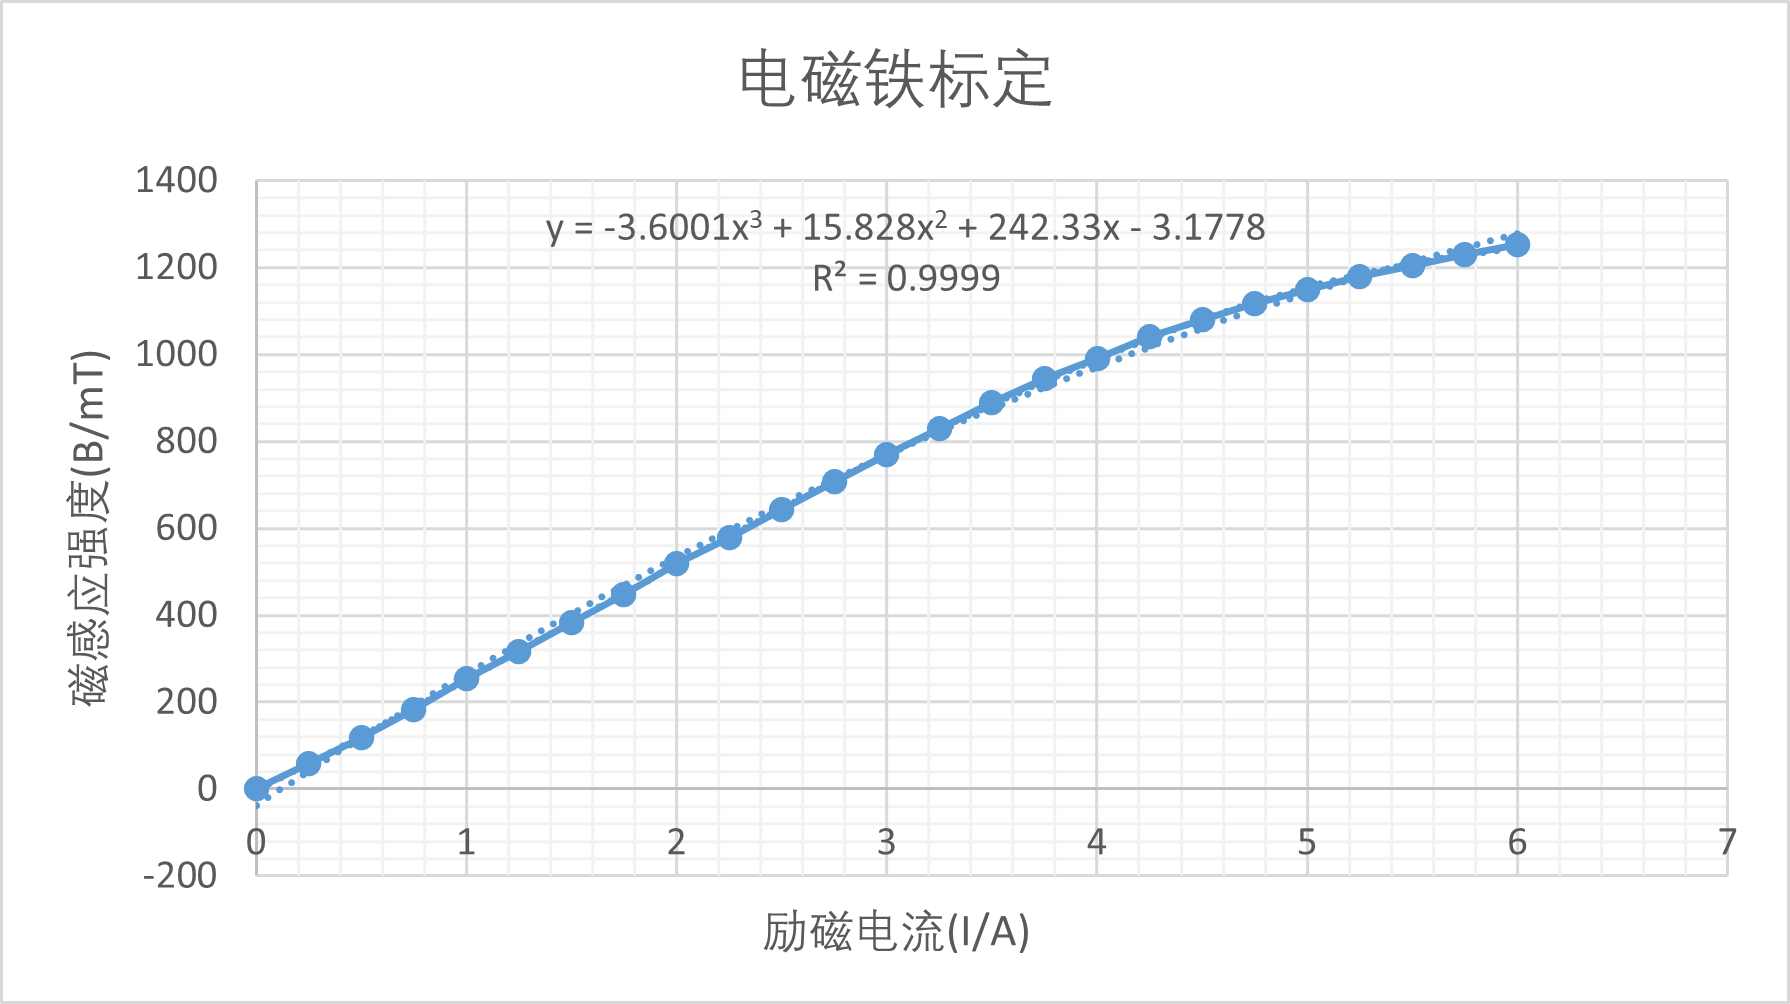
\includegraphics[width=0.65\textwidth]{磁场标定.png}
    \caption{励磁电流与磁场强度对应关系}
    \label{fig:current_magnetic}
\end{figure}

\subsubsection*{调节F-P标准具}
按照实验步骤中的方法，我们反复调节光路中各个元件的位置并通过CCD观察干涉条纹的清晰程度。
最终我们得到如图\ref{fig:FP}所示的干涉条纹。

\begin{figure}[h!]
    \centering
    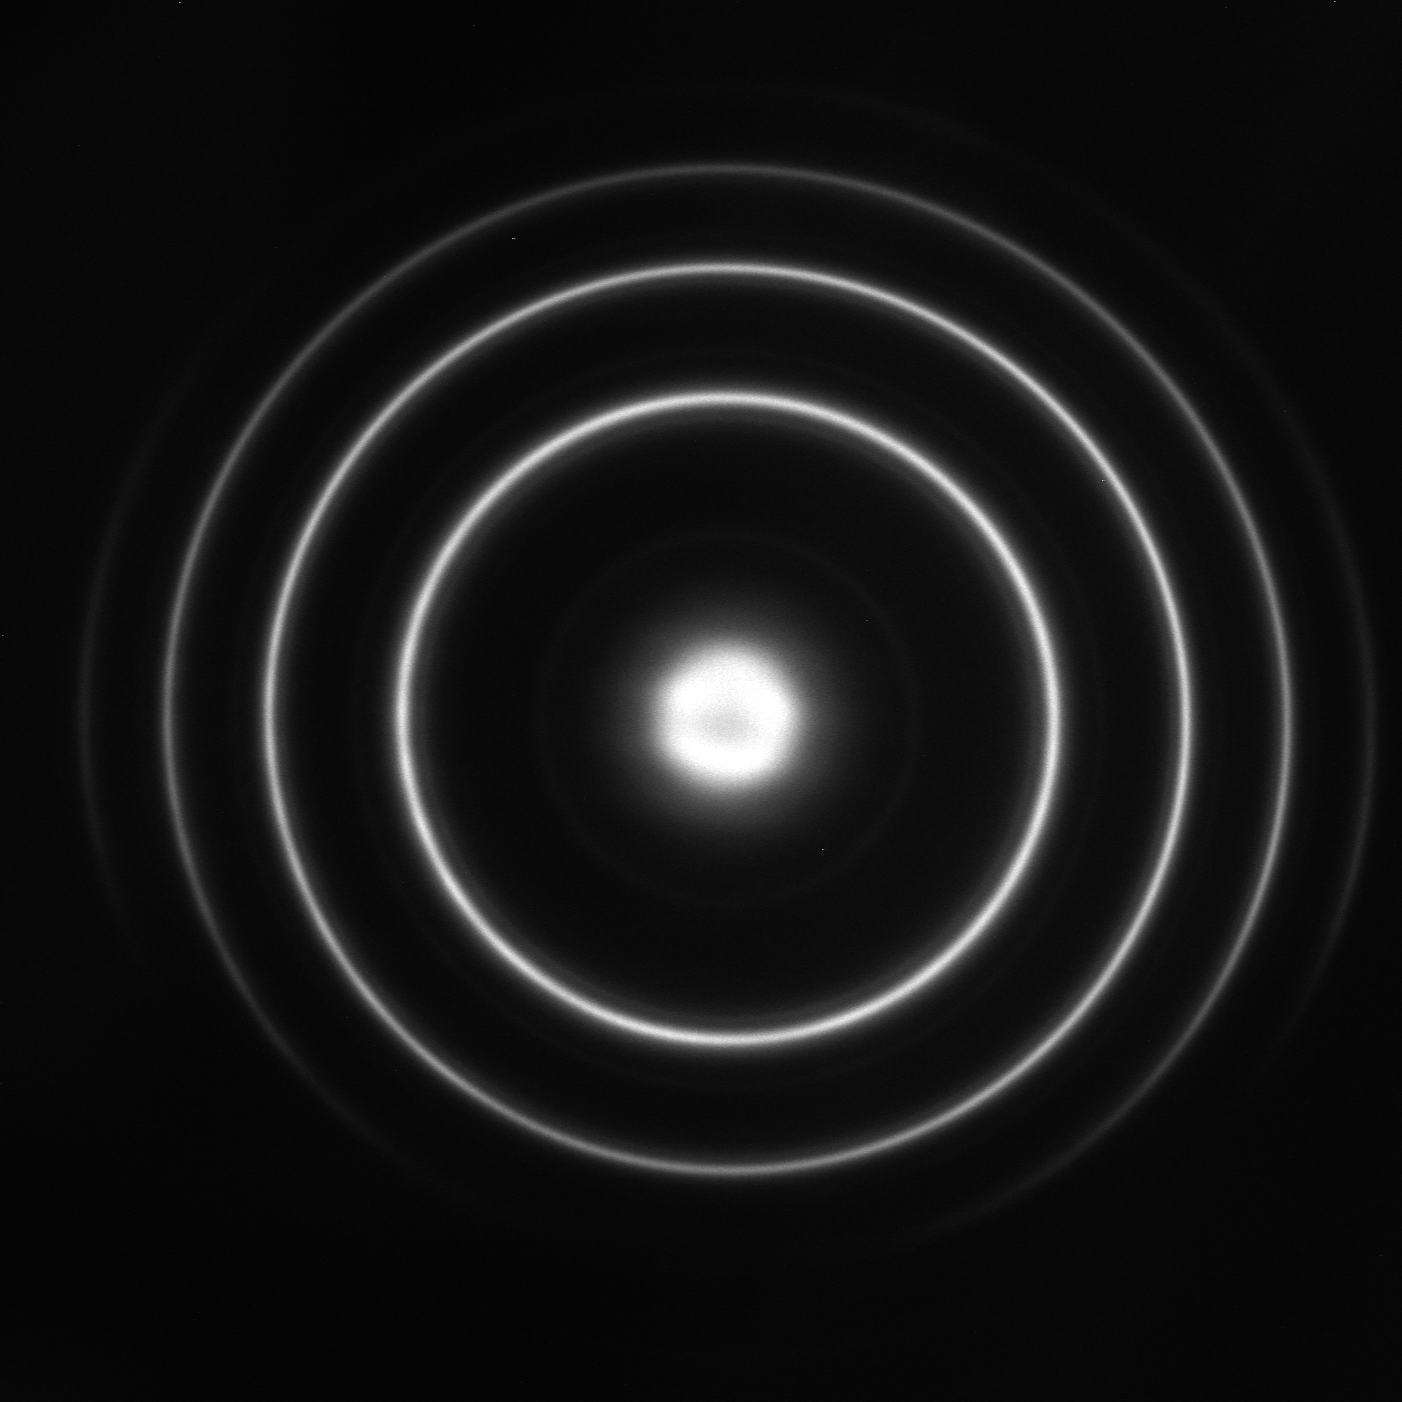
\includegraphics[width=0.65\textwidth]{F-P.png}
    \caption{F-P标准具干涉条纹}
    \label{fig:FP}
\end{figure}

可以看到清晰的干涉条纹。

\subsubsection*{调节偏振片角度}
观察到清晰的干涉条纹之后，适当添加磁场能够观察到各级干涉线的劈裂。
此时旋转偏振片的角度能够观察到干涉条纹发生明显的变化，这在一定程度上说明了产生的谱线的偏振特性。
我们多次改变偏振片的角度并记录CCD上的图像，确定最适合观察$\pi$线劈裂的偏振片角度。

\begin{figure}[h!]
    \centering
    \begin{minipage}[b]{0.3\textwidth}
        \centering
        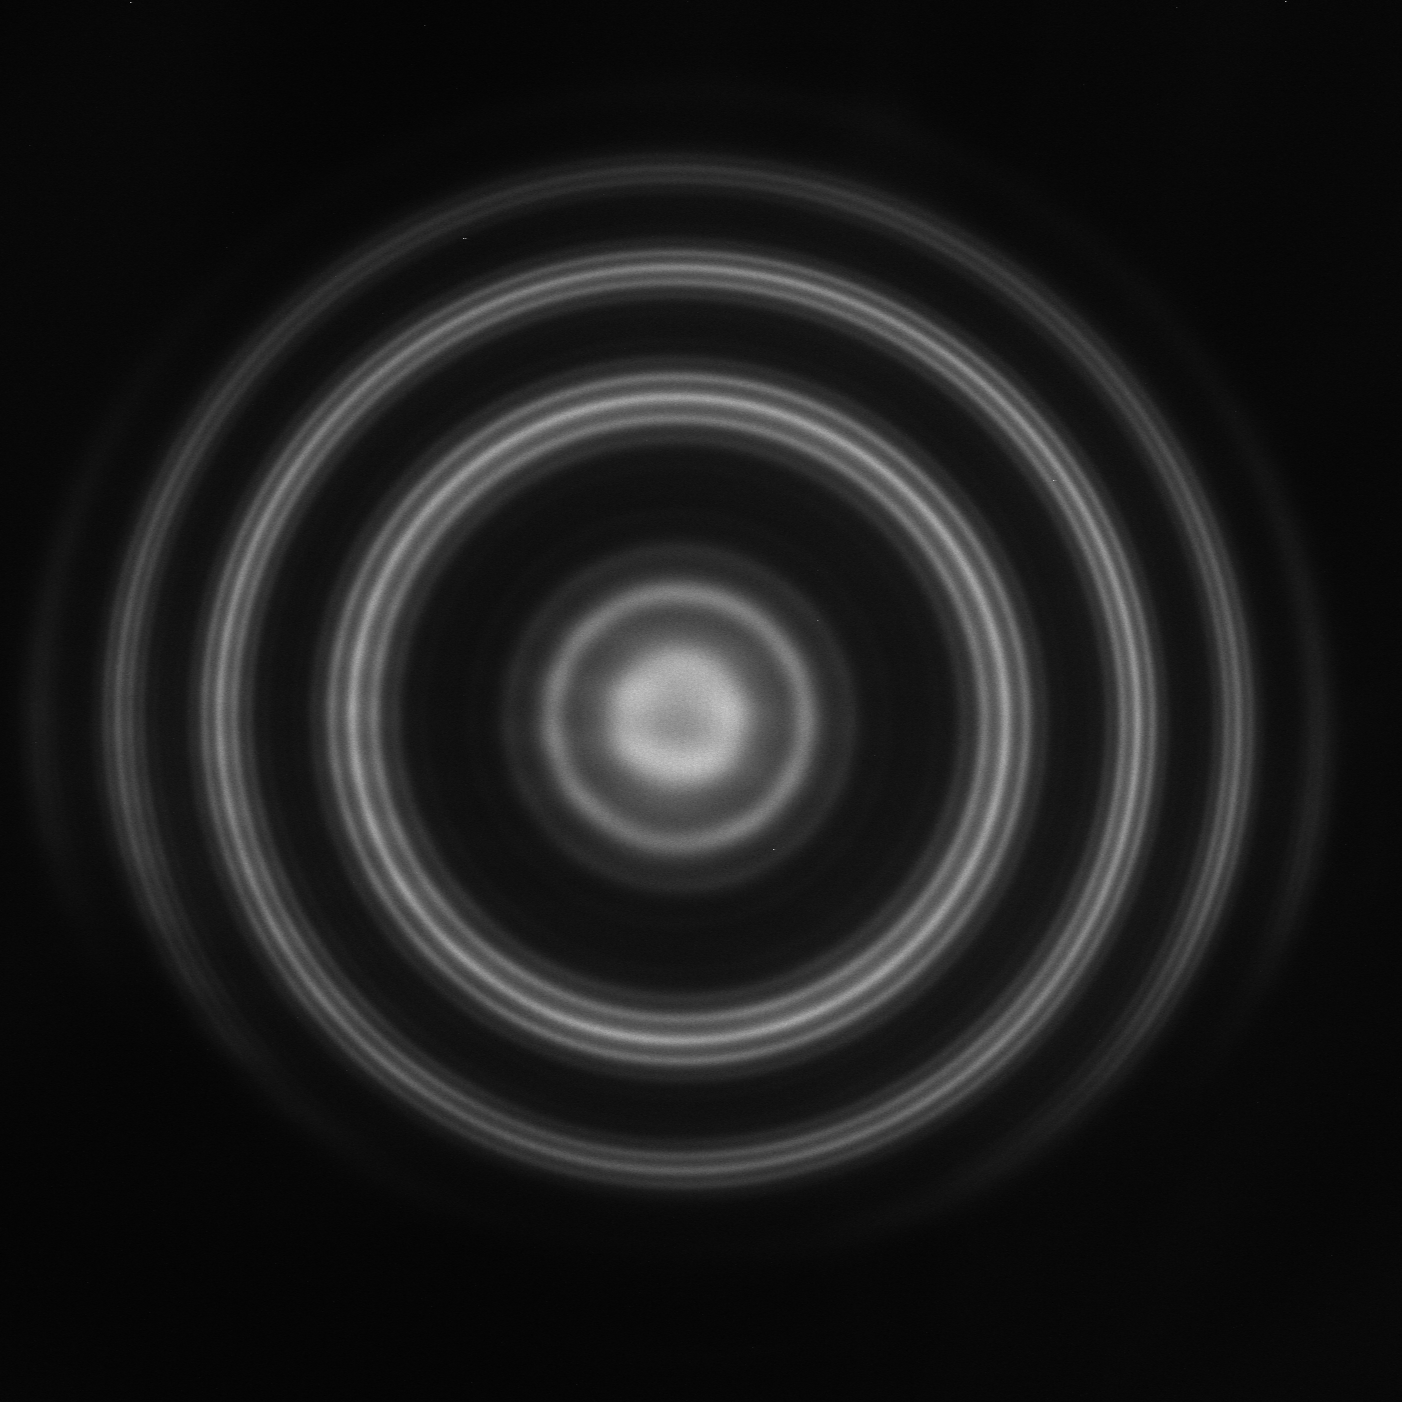
\includegraphics[width=\textwidth]{6.png}
        \caption{6°}
    \end{minipage}
    \begin{minipage}[b]{0.3\textwidth}
        \centering
        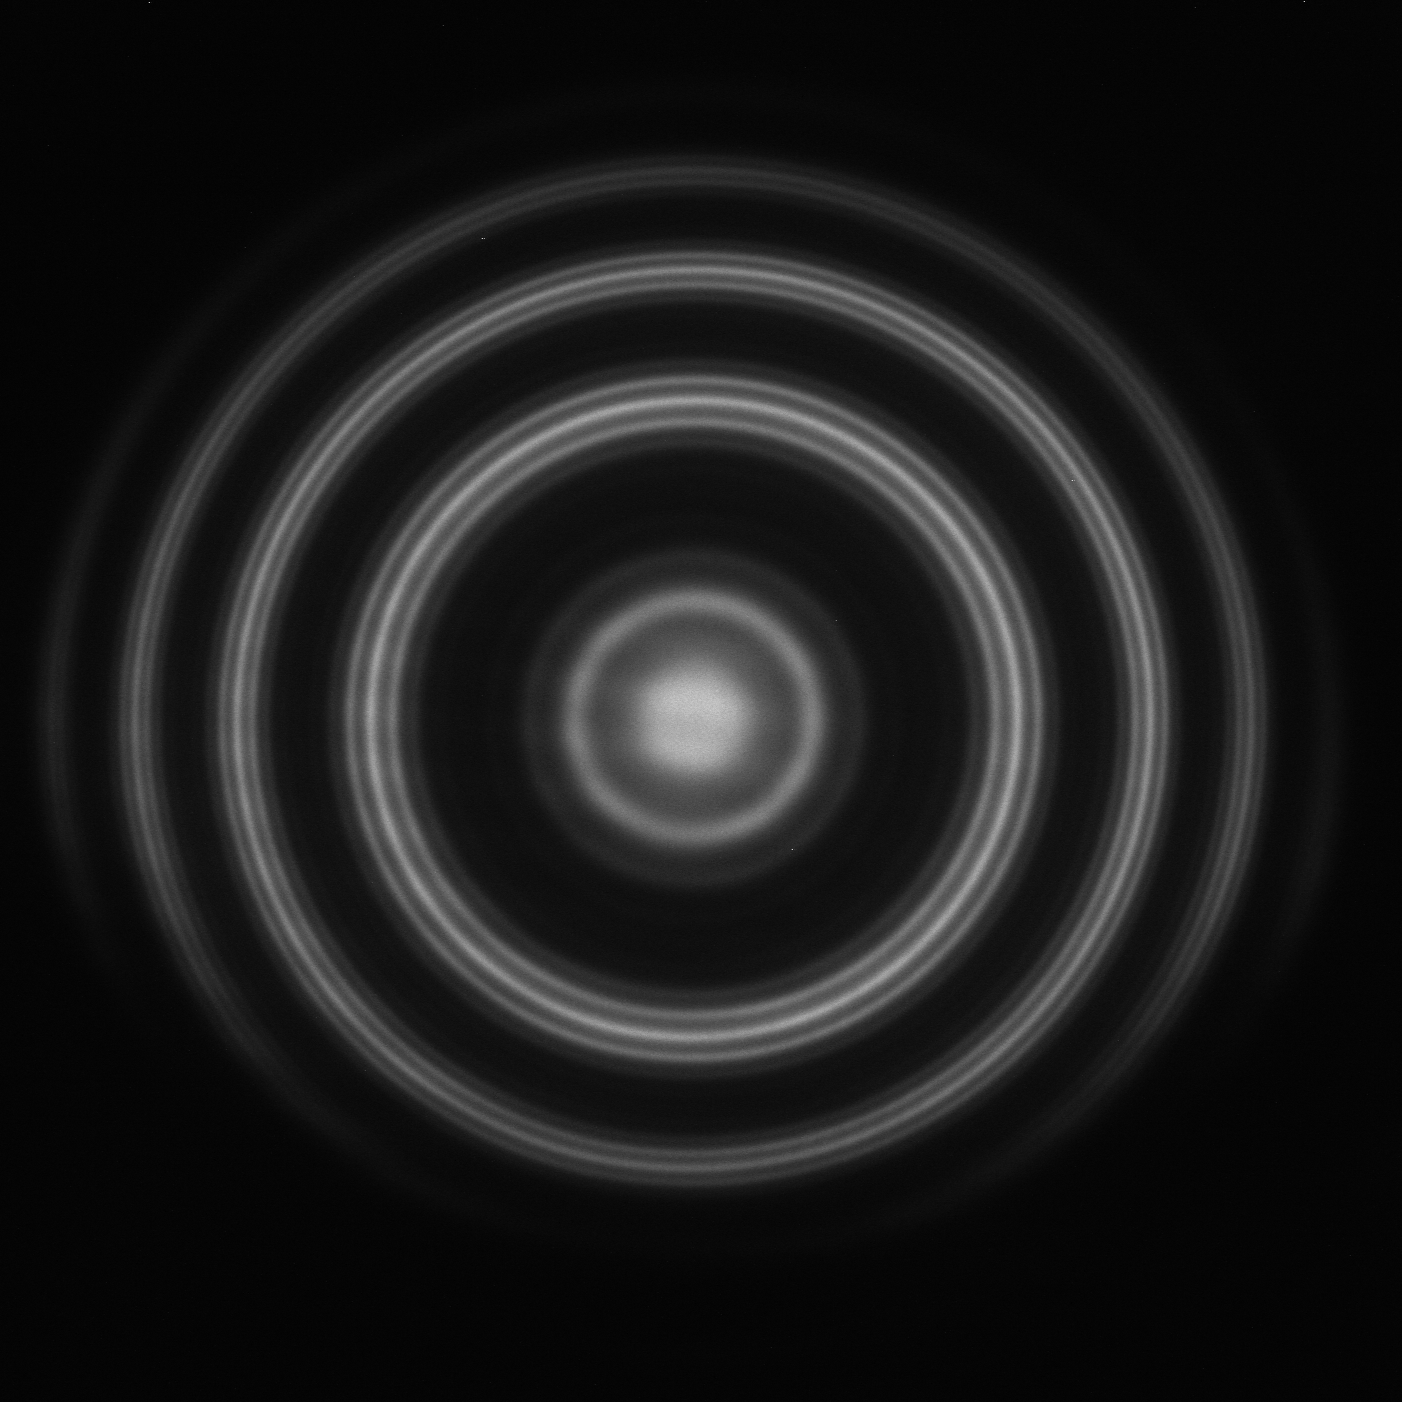
\includegraphics[width=\textwidth]{26.png}
        \caption{26°}
    \end{minipage}
    \begin{minipage}[b]{0.3\textwidth}
        \centering
        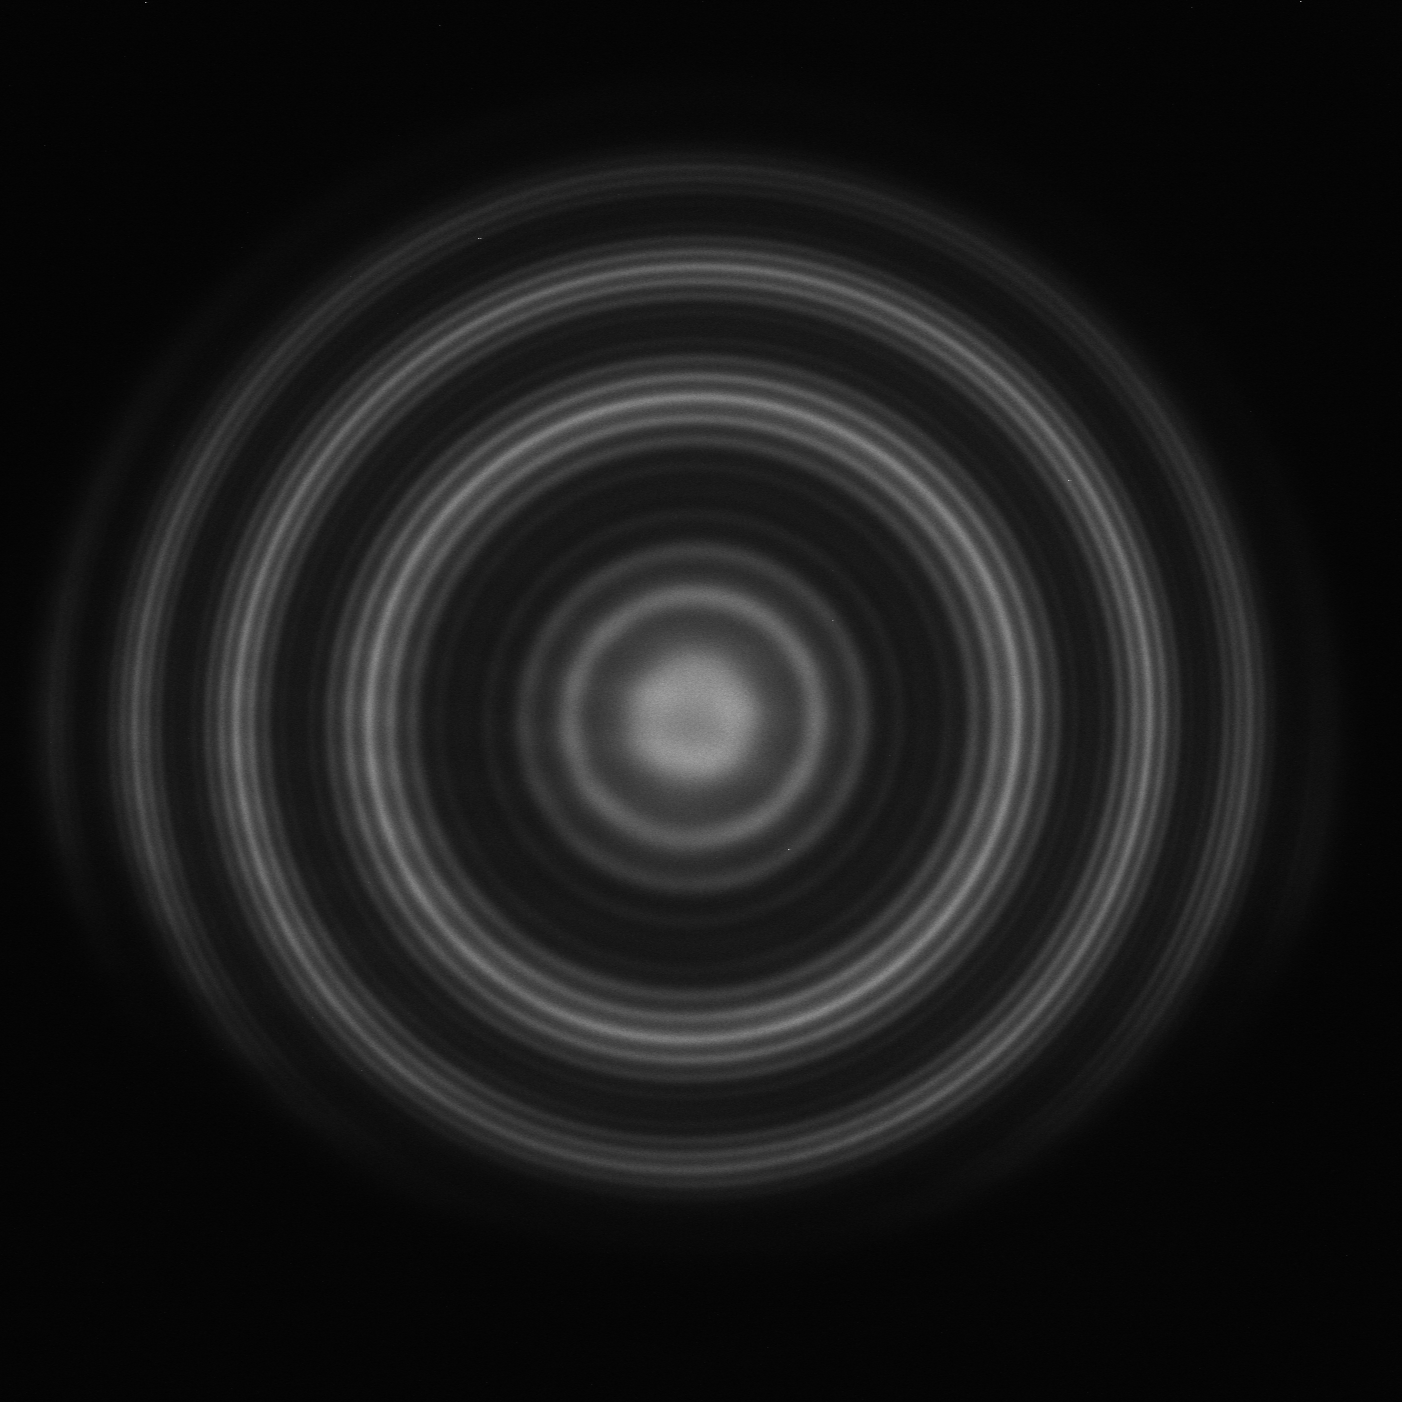
\includegraphics[width=\textwidth]{46.png}
        \caption{46°}
    \end{minipage}
    \begin{minipage}[b]{0.3\textwidth}
        \centering
        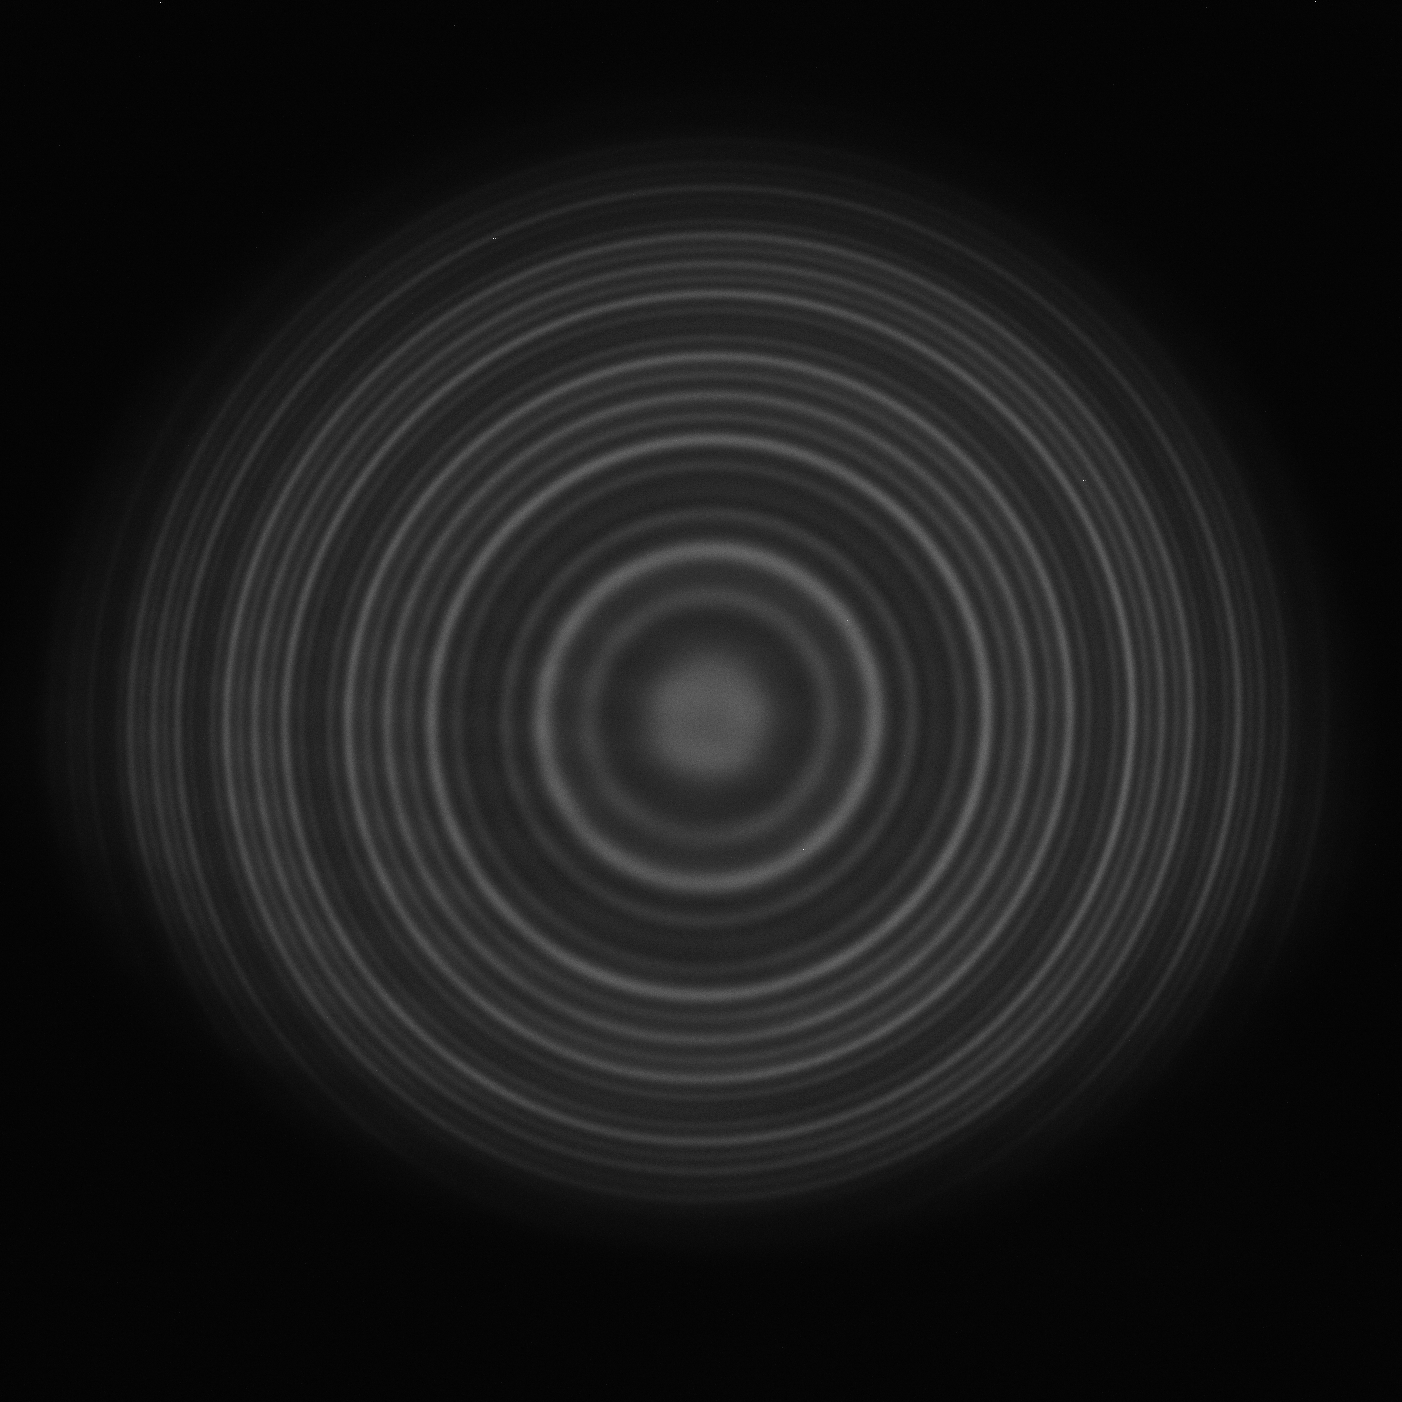
\includegraphics[width=\textwidth]{66.png}
        \caption{66°}
    \end{minipage}
    \begin{minipage}[b]{0.3\textwidth}
        \centering
        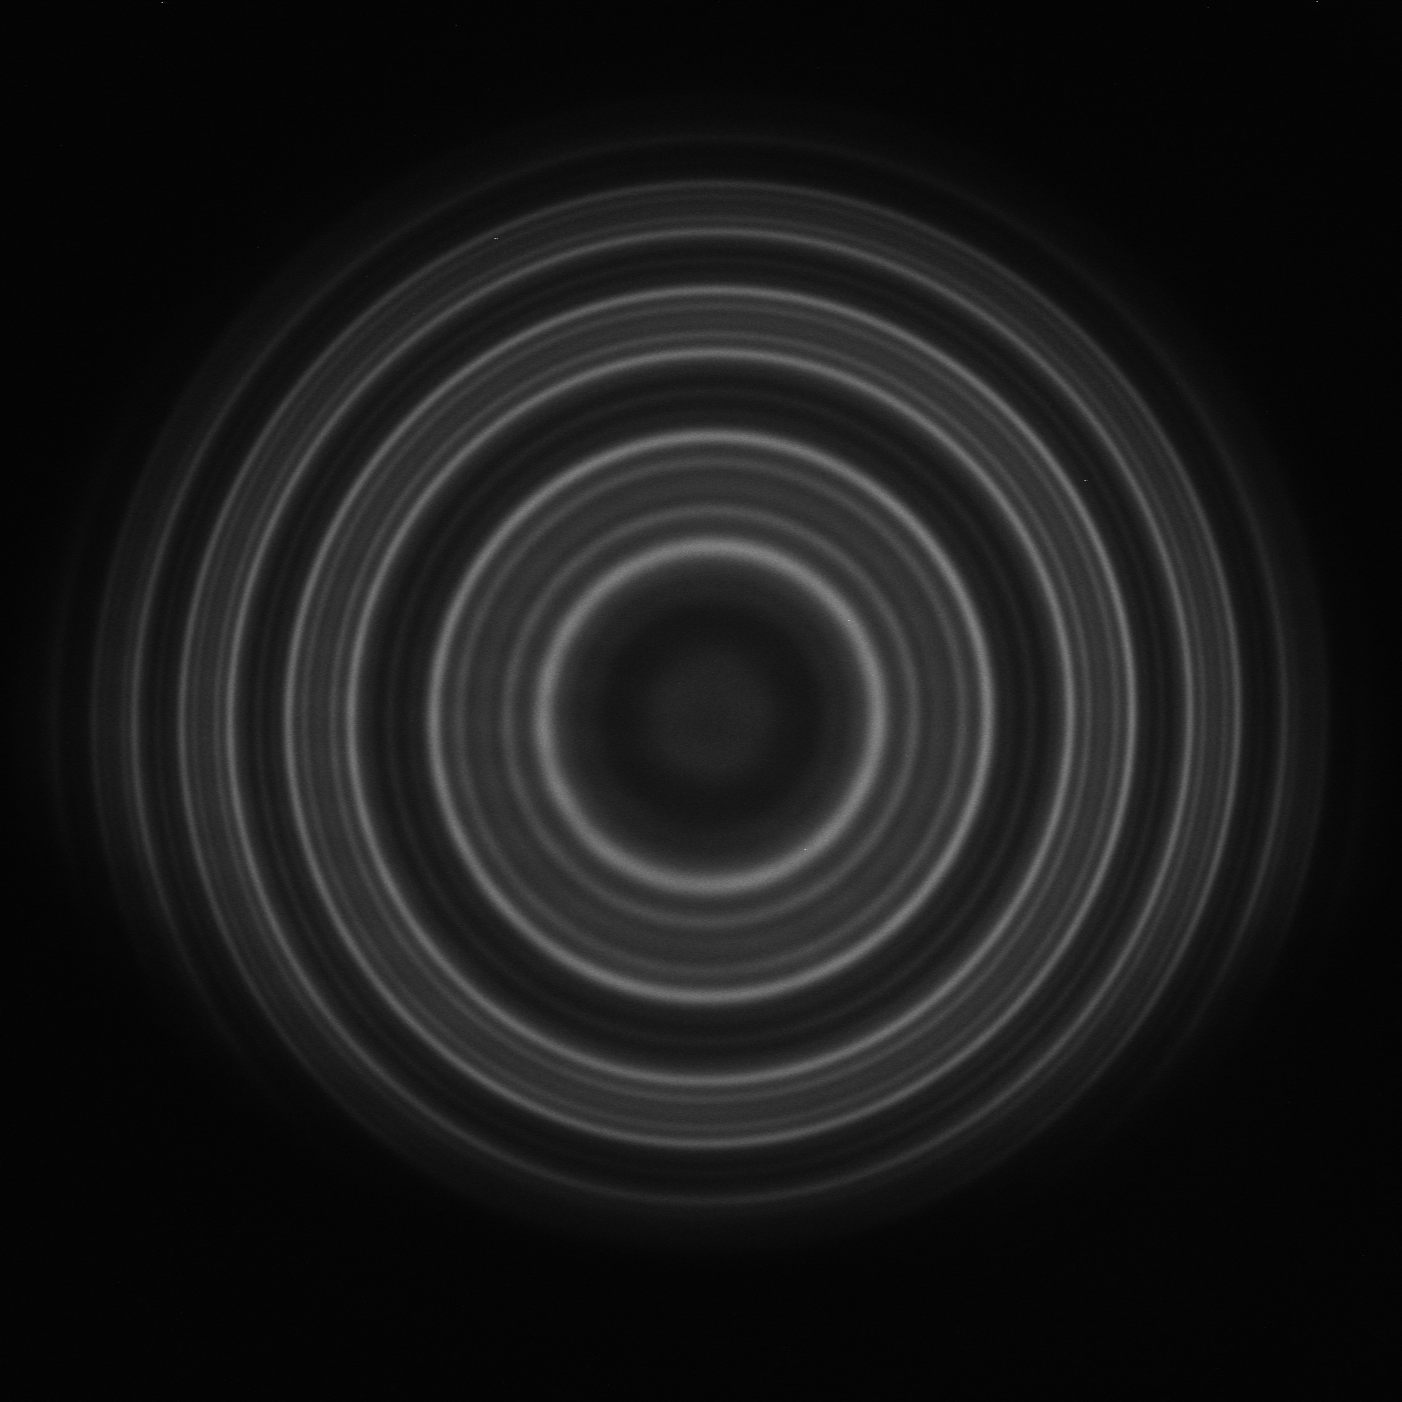
\includegraphics[width=\textwidth]{86.png}
        \caption{86°}
    \end{minipage}
    \begin{minipage}[b]{0.3\textwidth}
        \centering
        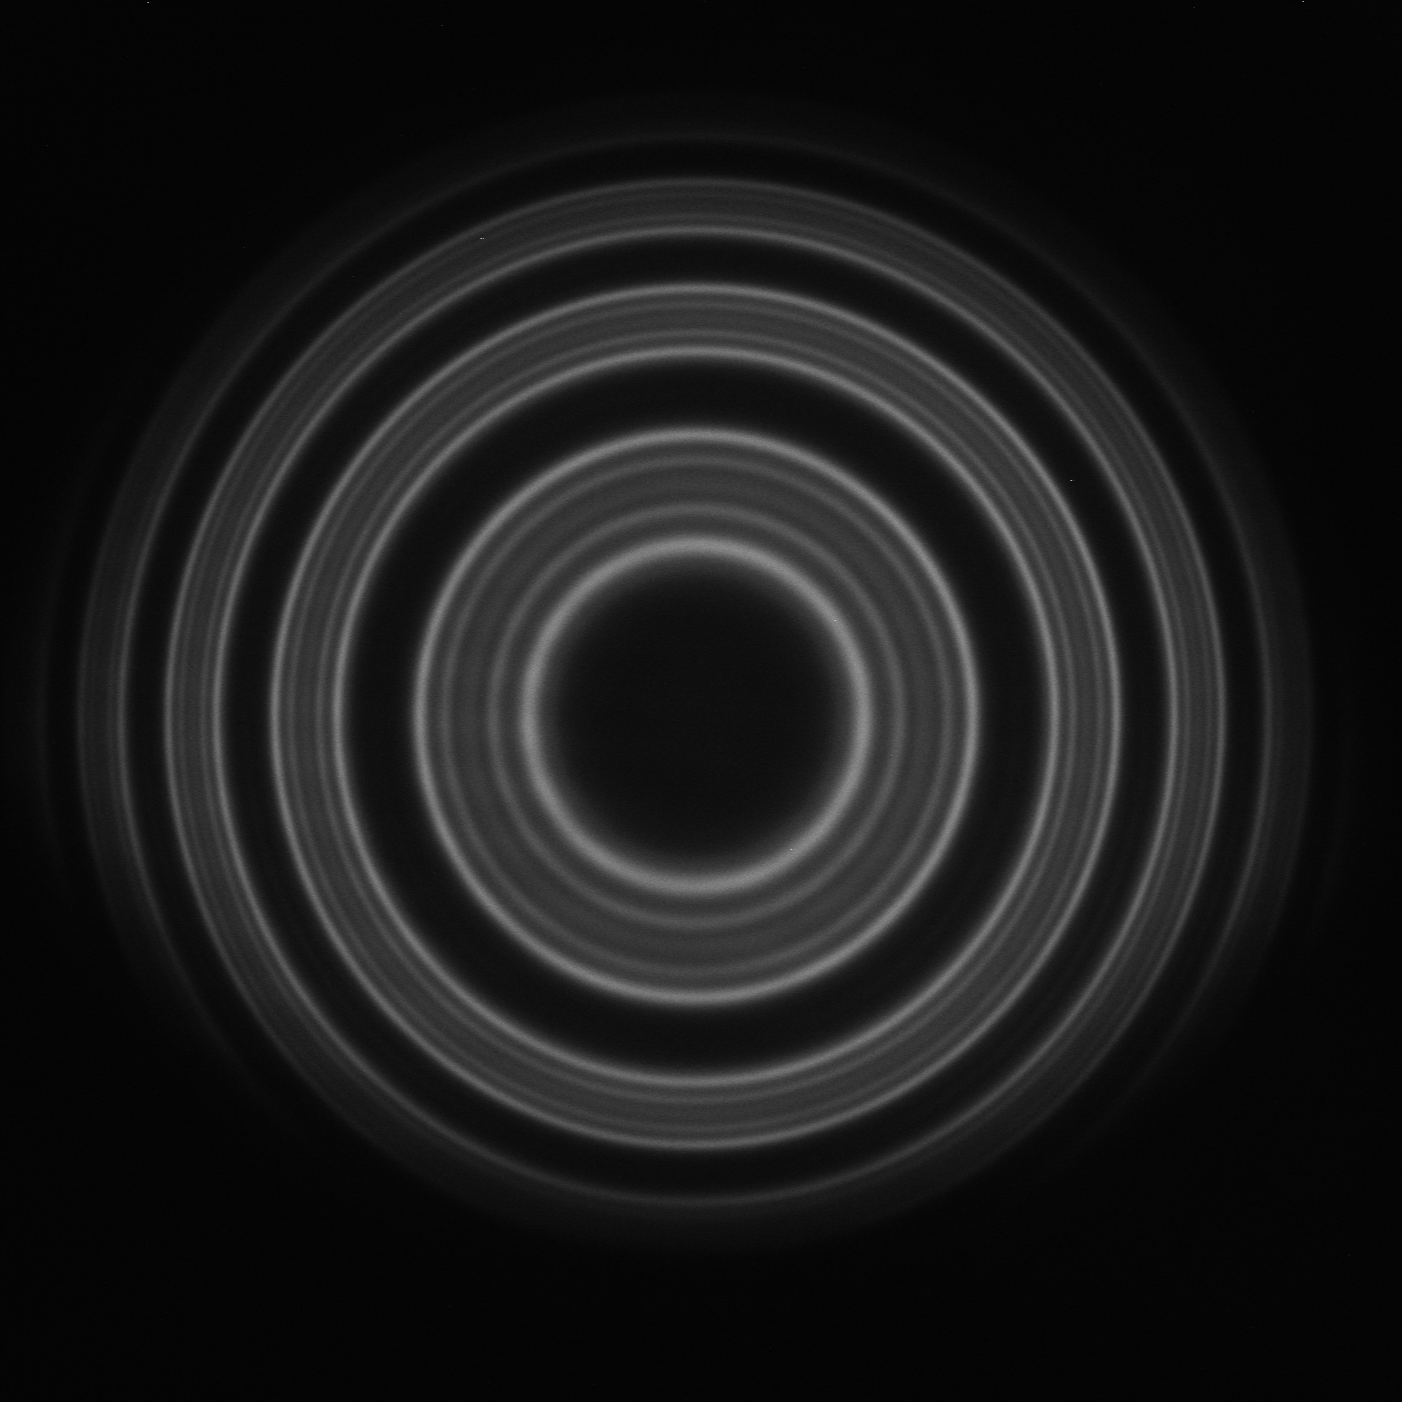
\includegraphics[width=\textwidth]{106.png}
        \caption{106°}
    \end{minipage}
    \begin{minipage}[b]{0.3\textwidth}
        \centering
        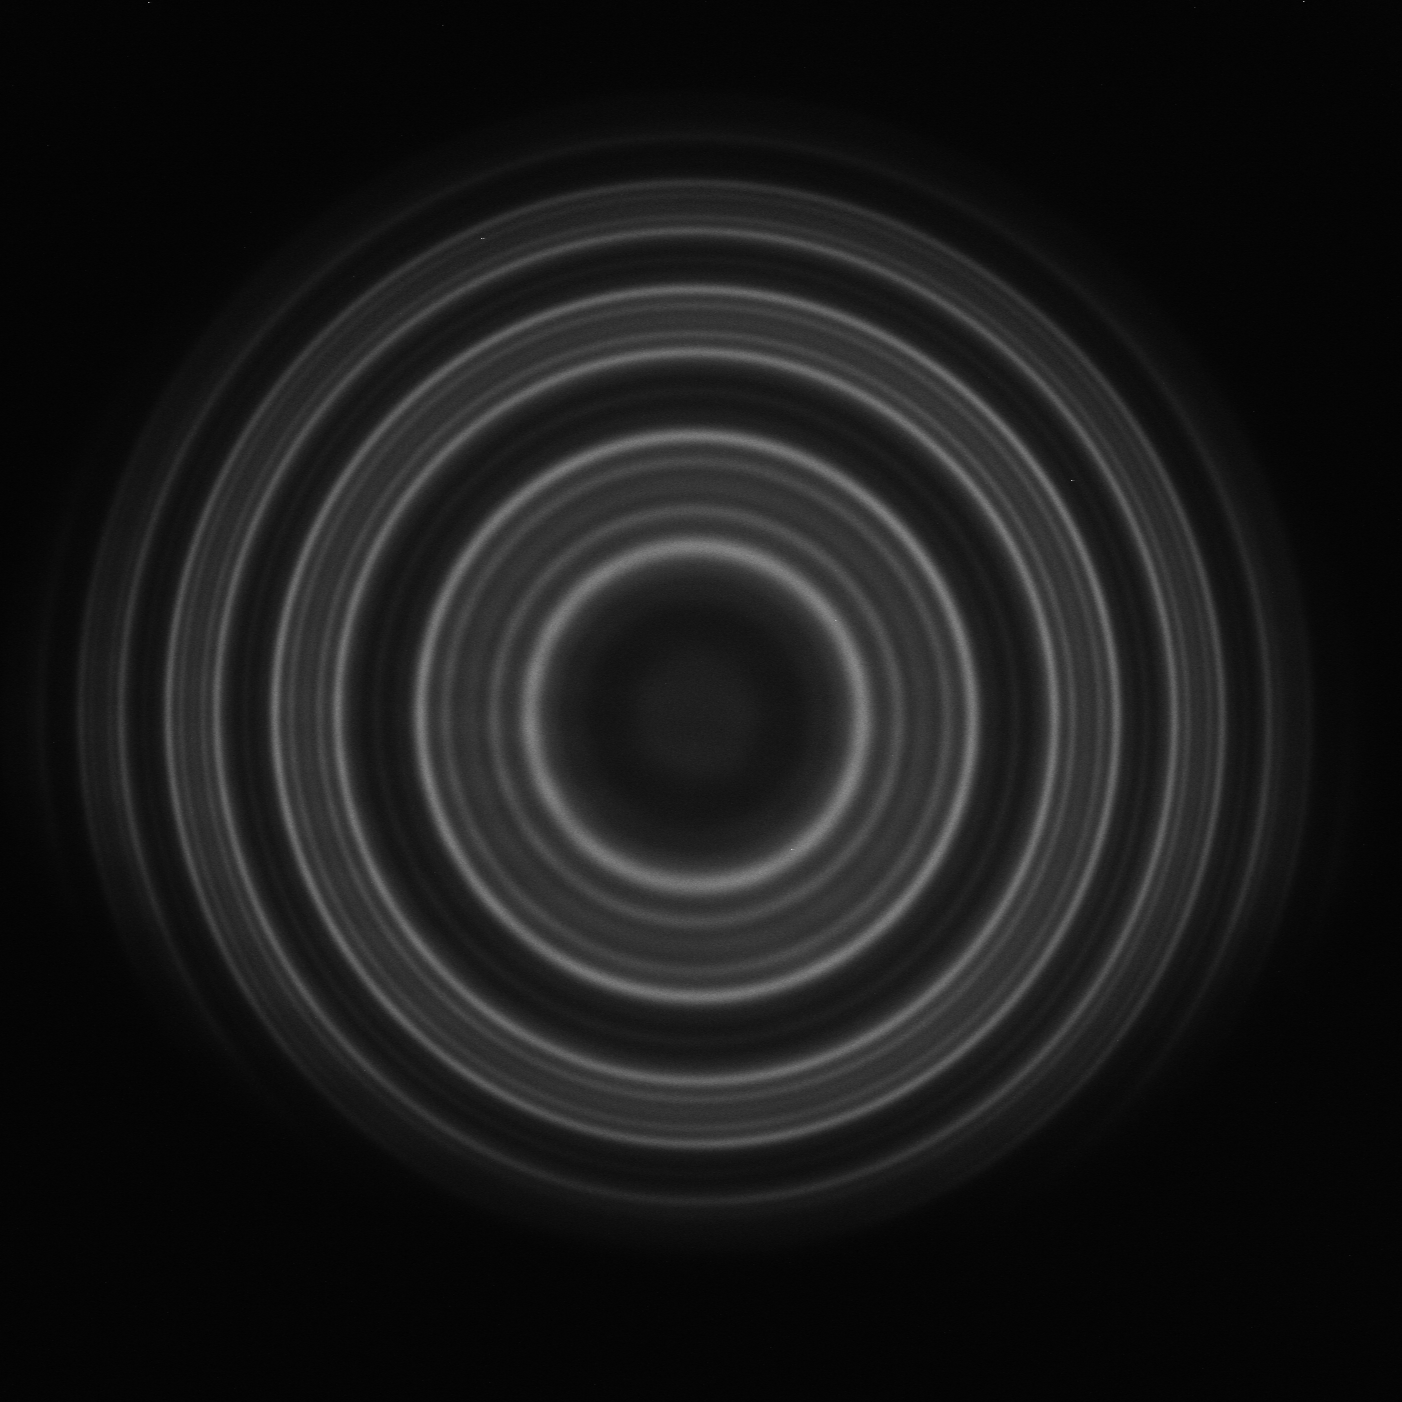
\includegraphics[width=\textwidth]{126.png}
        \caption{126°}
    \end{minipage}
    \begin{minipage}[b]{0.3\textwidth}
        \centering
        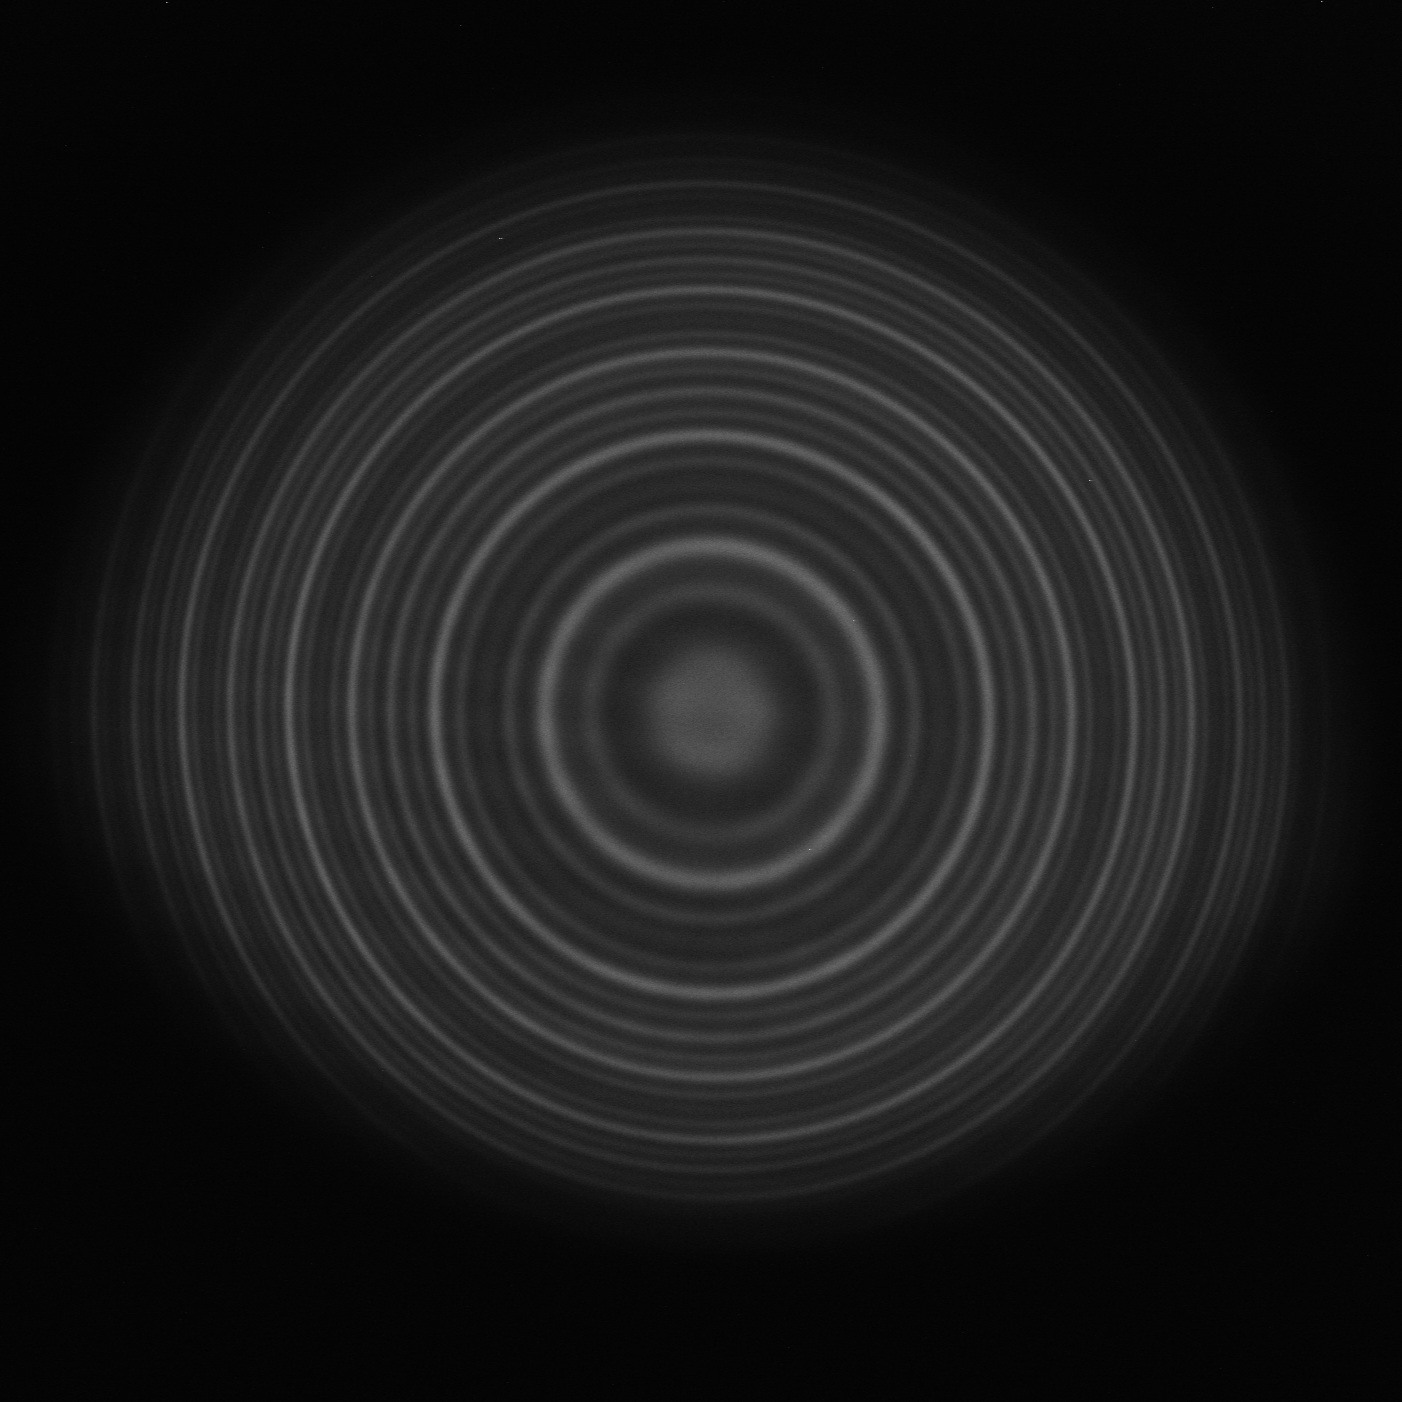
\includegraphics[width=\textwidth]{146.png}
        \caption{146°}
    \end{minipage}
    \begin{minipage}[b]{0.3\textwidth}
        \centering
        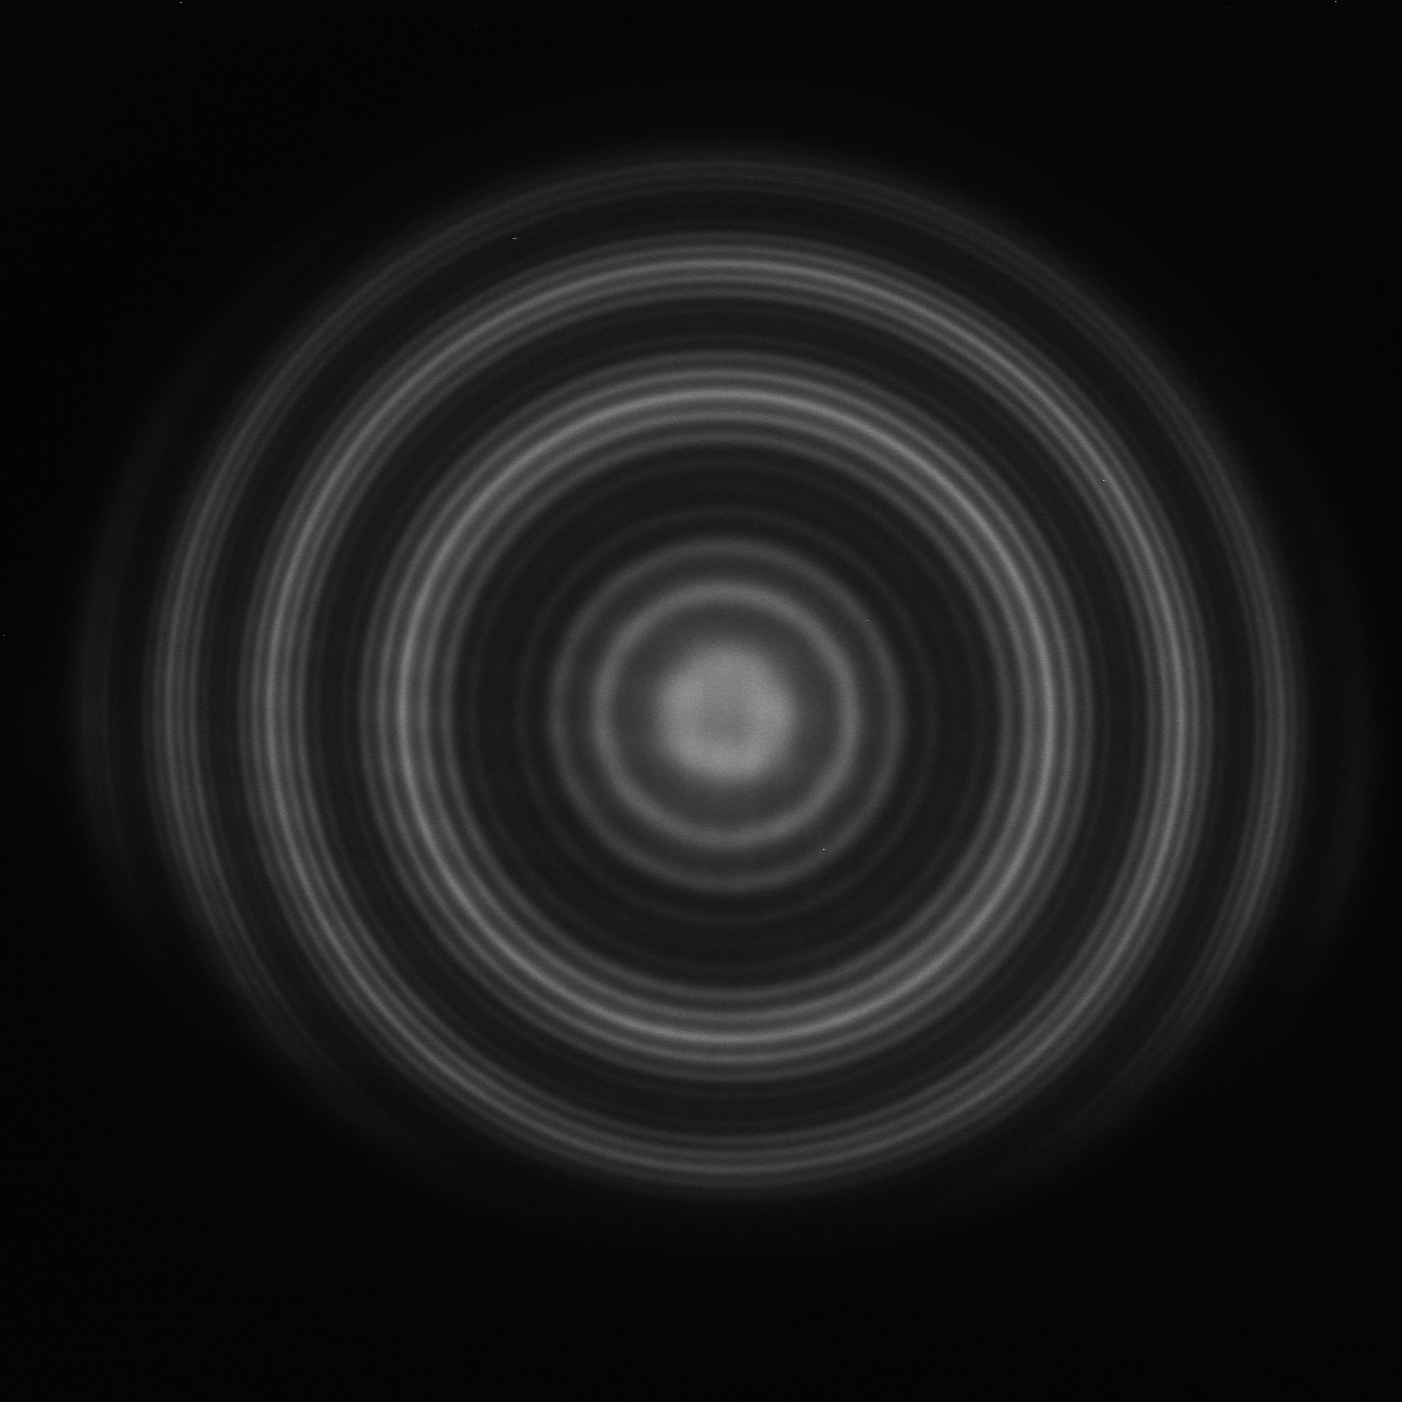
\includegraphics[width=\textwidth]{166.png}
        \caption{166°}
    \end{minipage}
    \caption{不同偏振片角度下的干涉条纹}
    \label{fig:polarization}
\end{figure}

由上图可见，最适合观察的偏振片角度再$6^\circ$左右，此时$\pi$线劈裂最为清晰。

\subsubsection*{观察反常塞曼效应}
调整偏振片的方向至$6^\circ$，使得线偏振光的劈裂在CCD上显示最为明显。
随后我们可以开始观察塞曼效应，我们在$0-6A$范围内选取了四个电流值，分别为$0A,2A,4A,6A$。
记录下每个电流值对应的谱线劈裂情况，并保存CCD中看到的图像，结果如图\ref{fig:ZeemanI}所示。

此时能够看到原先F-P标准具的谱线劈裂为三条，且随着电流的增大，谱线分裂程度也逐渐大。

\begin{figure}[h!]
    \centering
    \begin{minipage}[b]{0.48\textwidth}
        \centering
        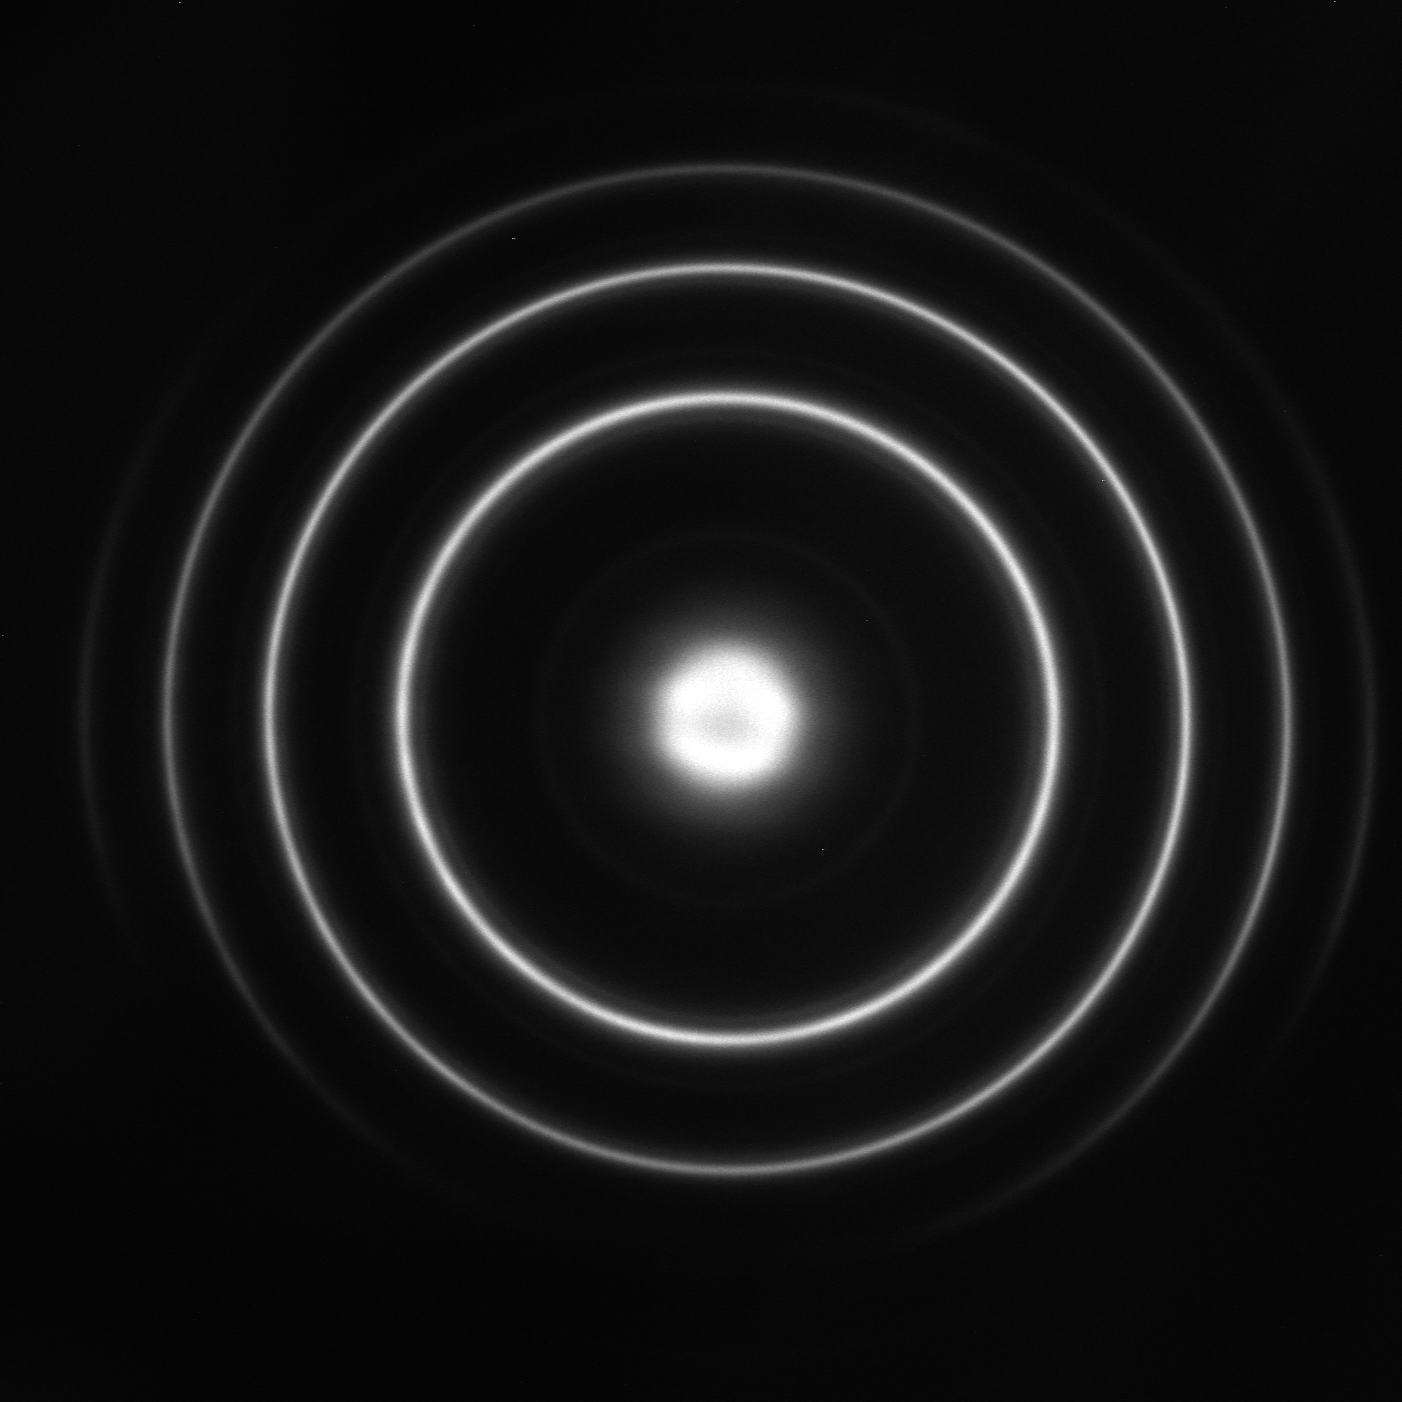
\includegraphics[width=\textwidth]{0.png}
        \caption{0A}
    \end{minipage}
    \begin{minipage}[b]{0.48\textwidth}
        \centering
        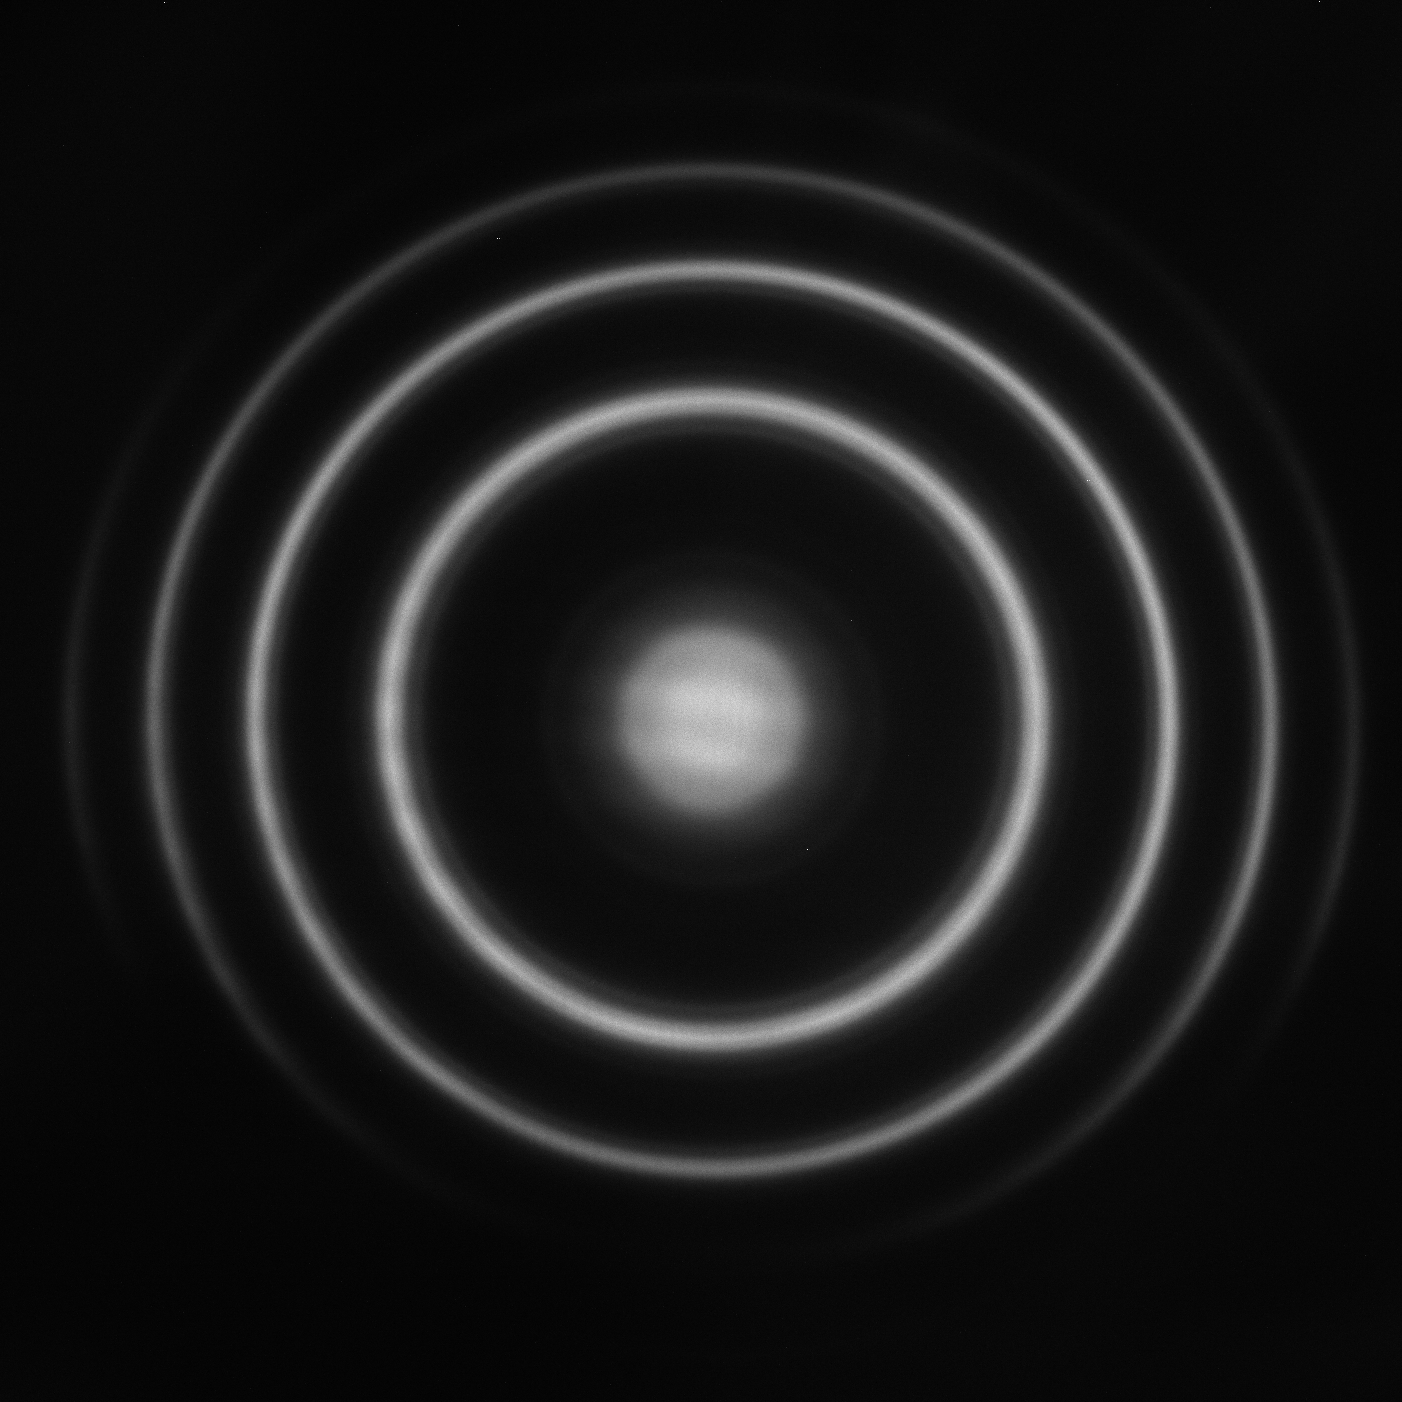
\includegraphics[width=\textwidth]{2.png}
        \caption{2A}
    \end{minipage}
    \begin{minipage}[b]{0.48\textwidth}
        \centering
        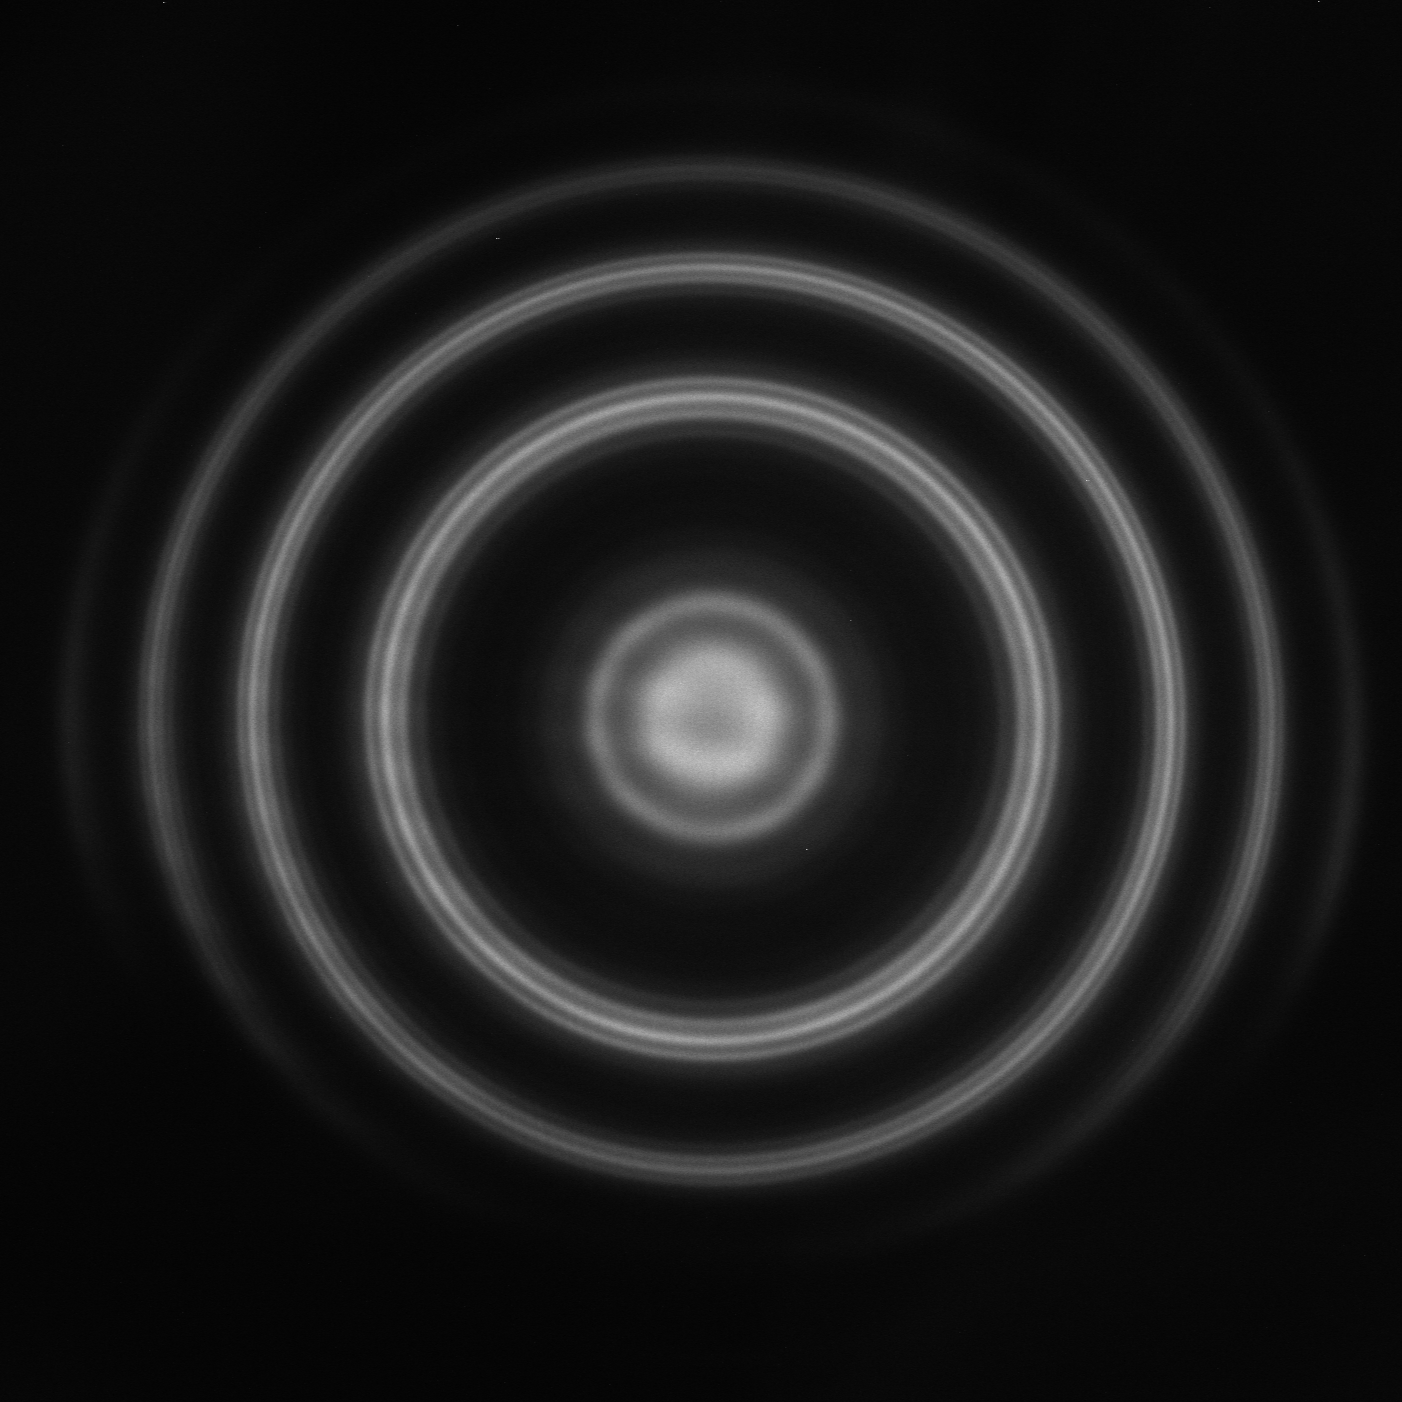
\includegraphics[width=\textwidth]{4.png}
        \caption{4A}
    \end{minipage}
    \begin{minipage}[b]{0.48\textwidth}
        \centering
        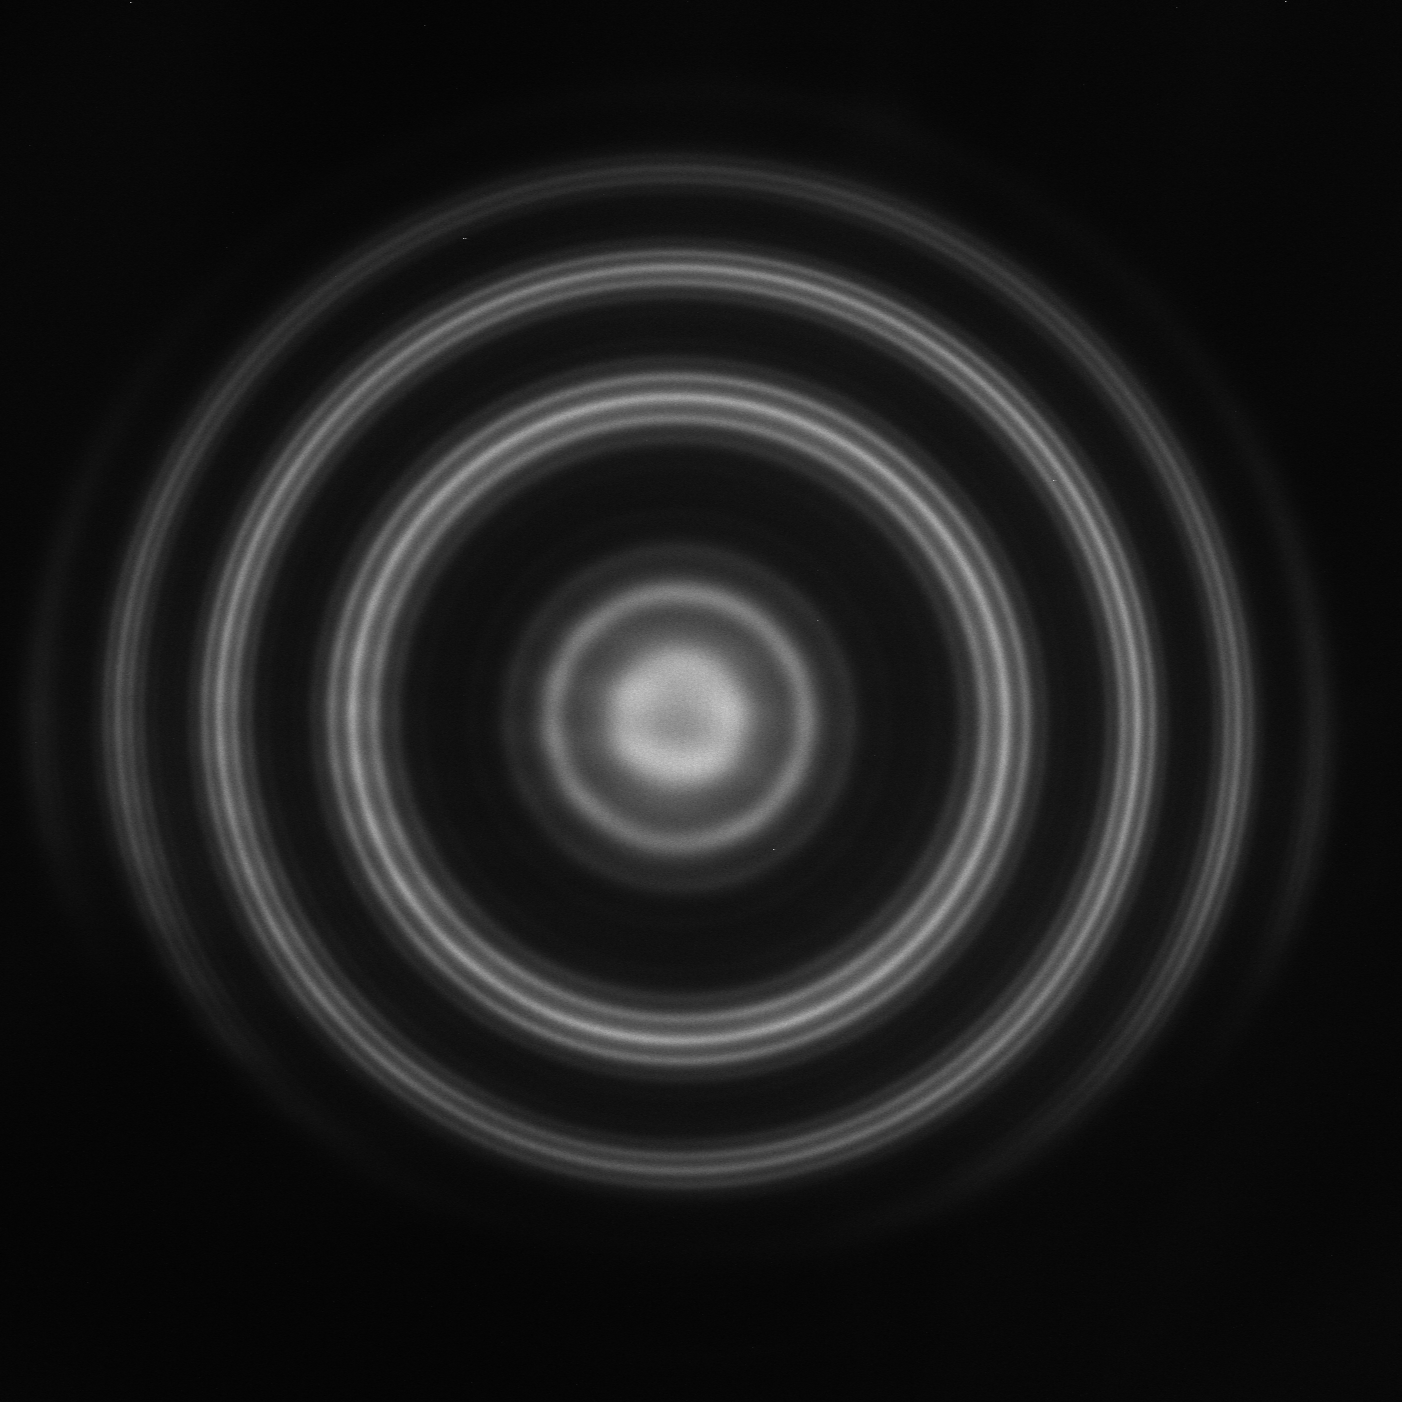
\includegraphics[width=\textwidth]{6.png}
        \caption{6A}
    \end{minipage}
    \caption{不同电流值下的塞曼效应}
    \label{fig:ZeemanI}
\end{figure}

\subsubsection*{通过在CCD上测量谱线的劈裂来计算荷质比}
从前面的实验原理部分我们可以知道，荷质比的计算公式为：
\begin{equation}
    \frac{e}{m} = \frac{2\pi c}{d \, B \left(M_{2}g_{2}-M_{1}g_{1}\right)} \, \frac{D_{b}^{2}-D_{a}^{2}}{D_{N-1}^{2}-D_{N}^{2}}
\end{equation}

其中$c$为光速，$d$为F-P标准具的厚度，$B$为磁场强度，$g_{1}，g_{2}$为朗德因子，$D_{b}$ $D_{a}$ $D_{N-1}$ $D_{N}$为CCD上测得的劈裂谱线半径。

此处我们测量的两条谱线对应的$g_{2}-g_{1}=\frac{1}{2}$，因此我们只需要测量出劈裂谱线半径即可。
这里值得注意的是我们在使用CCD时并未对CCD像素点之间的距离进行标定，但是由于计算公式中，圆环半径$D$的量纲回互相抵消，所以我们只需要测量半径对应的像素点个数即可。

这里列举我们用到的参数的数值以便参考：
\begin{table}[h!]
    \centering
    \begin{tabular}{cc}
        \hline
        参数 & 数值 \\
        \hline
        光速 $c$ & $2.997 \times 10^8 \mathrm{m/s}$ \\
        F-P标准具厚度 $d$ & $2.05 \mathrm{mm}$ \\
        参考值 $e/m$  & $1.7588 \times 10^{11} \mathrm{C/kg}$ \\
        \hline
    \end{tabular}
    \caption{实验参数}
    \label{tab:parameters}
\end{table}

我们在利用CCD配套的测量软件，在图像中添加十字坐标，并手动将坐标原点放置在F-P标准具的中心位置。
此时测量软件下方便能够显示光标所在位置对应的像素点坐标，我们将鼠标放置在不同圆环上，并记录对应的坐标，稍加处理便可以得到圆环的半径。
下面的表格呈现了在不同电流值下我们测量得到的劈裂谱线半径，以及按照上述公式计算得到的荷质比。

\begin{table}[h!]
    \centering
    \begin{tabular}{|c|c|c|c|c|c|c|}
        \hline
        电流(A) & 磁场(mT) & $D_a / D_N$(pix) & $D_b$(pix) & $D_{N-1}$(pix)  & $\cfrac{e}{m}(10^{11}\mathrm{C/kg})$ & 相对误差($\%$) \\
        \hline\hline
        5.788 & 1231.6 & 331 & 312 & 463 & 1.741 & 1.01$\%$ \\
        4.999 & 1154.0 & 335 & 317 & 464 & 1.814 & 1.28$\%$ \\
        4.499 & 1079.6 & 335 & 318 & 467 & 1.786 & 1.54$\%$ \\
        \hline
    \end{tabular}
    \caption{不同电流值下的测量数据}
    \label{tab:measurements}
\end{table}

可见我们的测量结果与参考值的相对误差在$1.5\%$左右，符合实验要求。

\textbf{第二周实验：观察正常塞曼效应}

\subsubsection*{光路和滤波片调节}
在继续进行实验之前我们需要重新调节塞曼效应的测量光路，具体的方法和过程和上周相同，这里不在赘述。

\begin{figure}[h!]
    \centering
    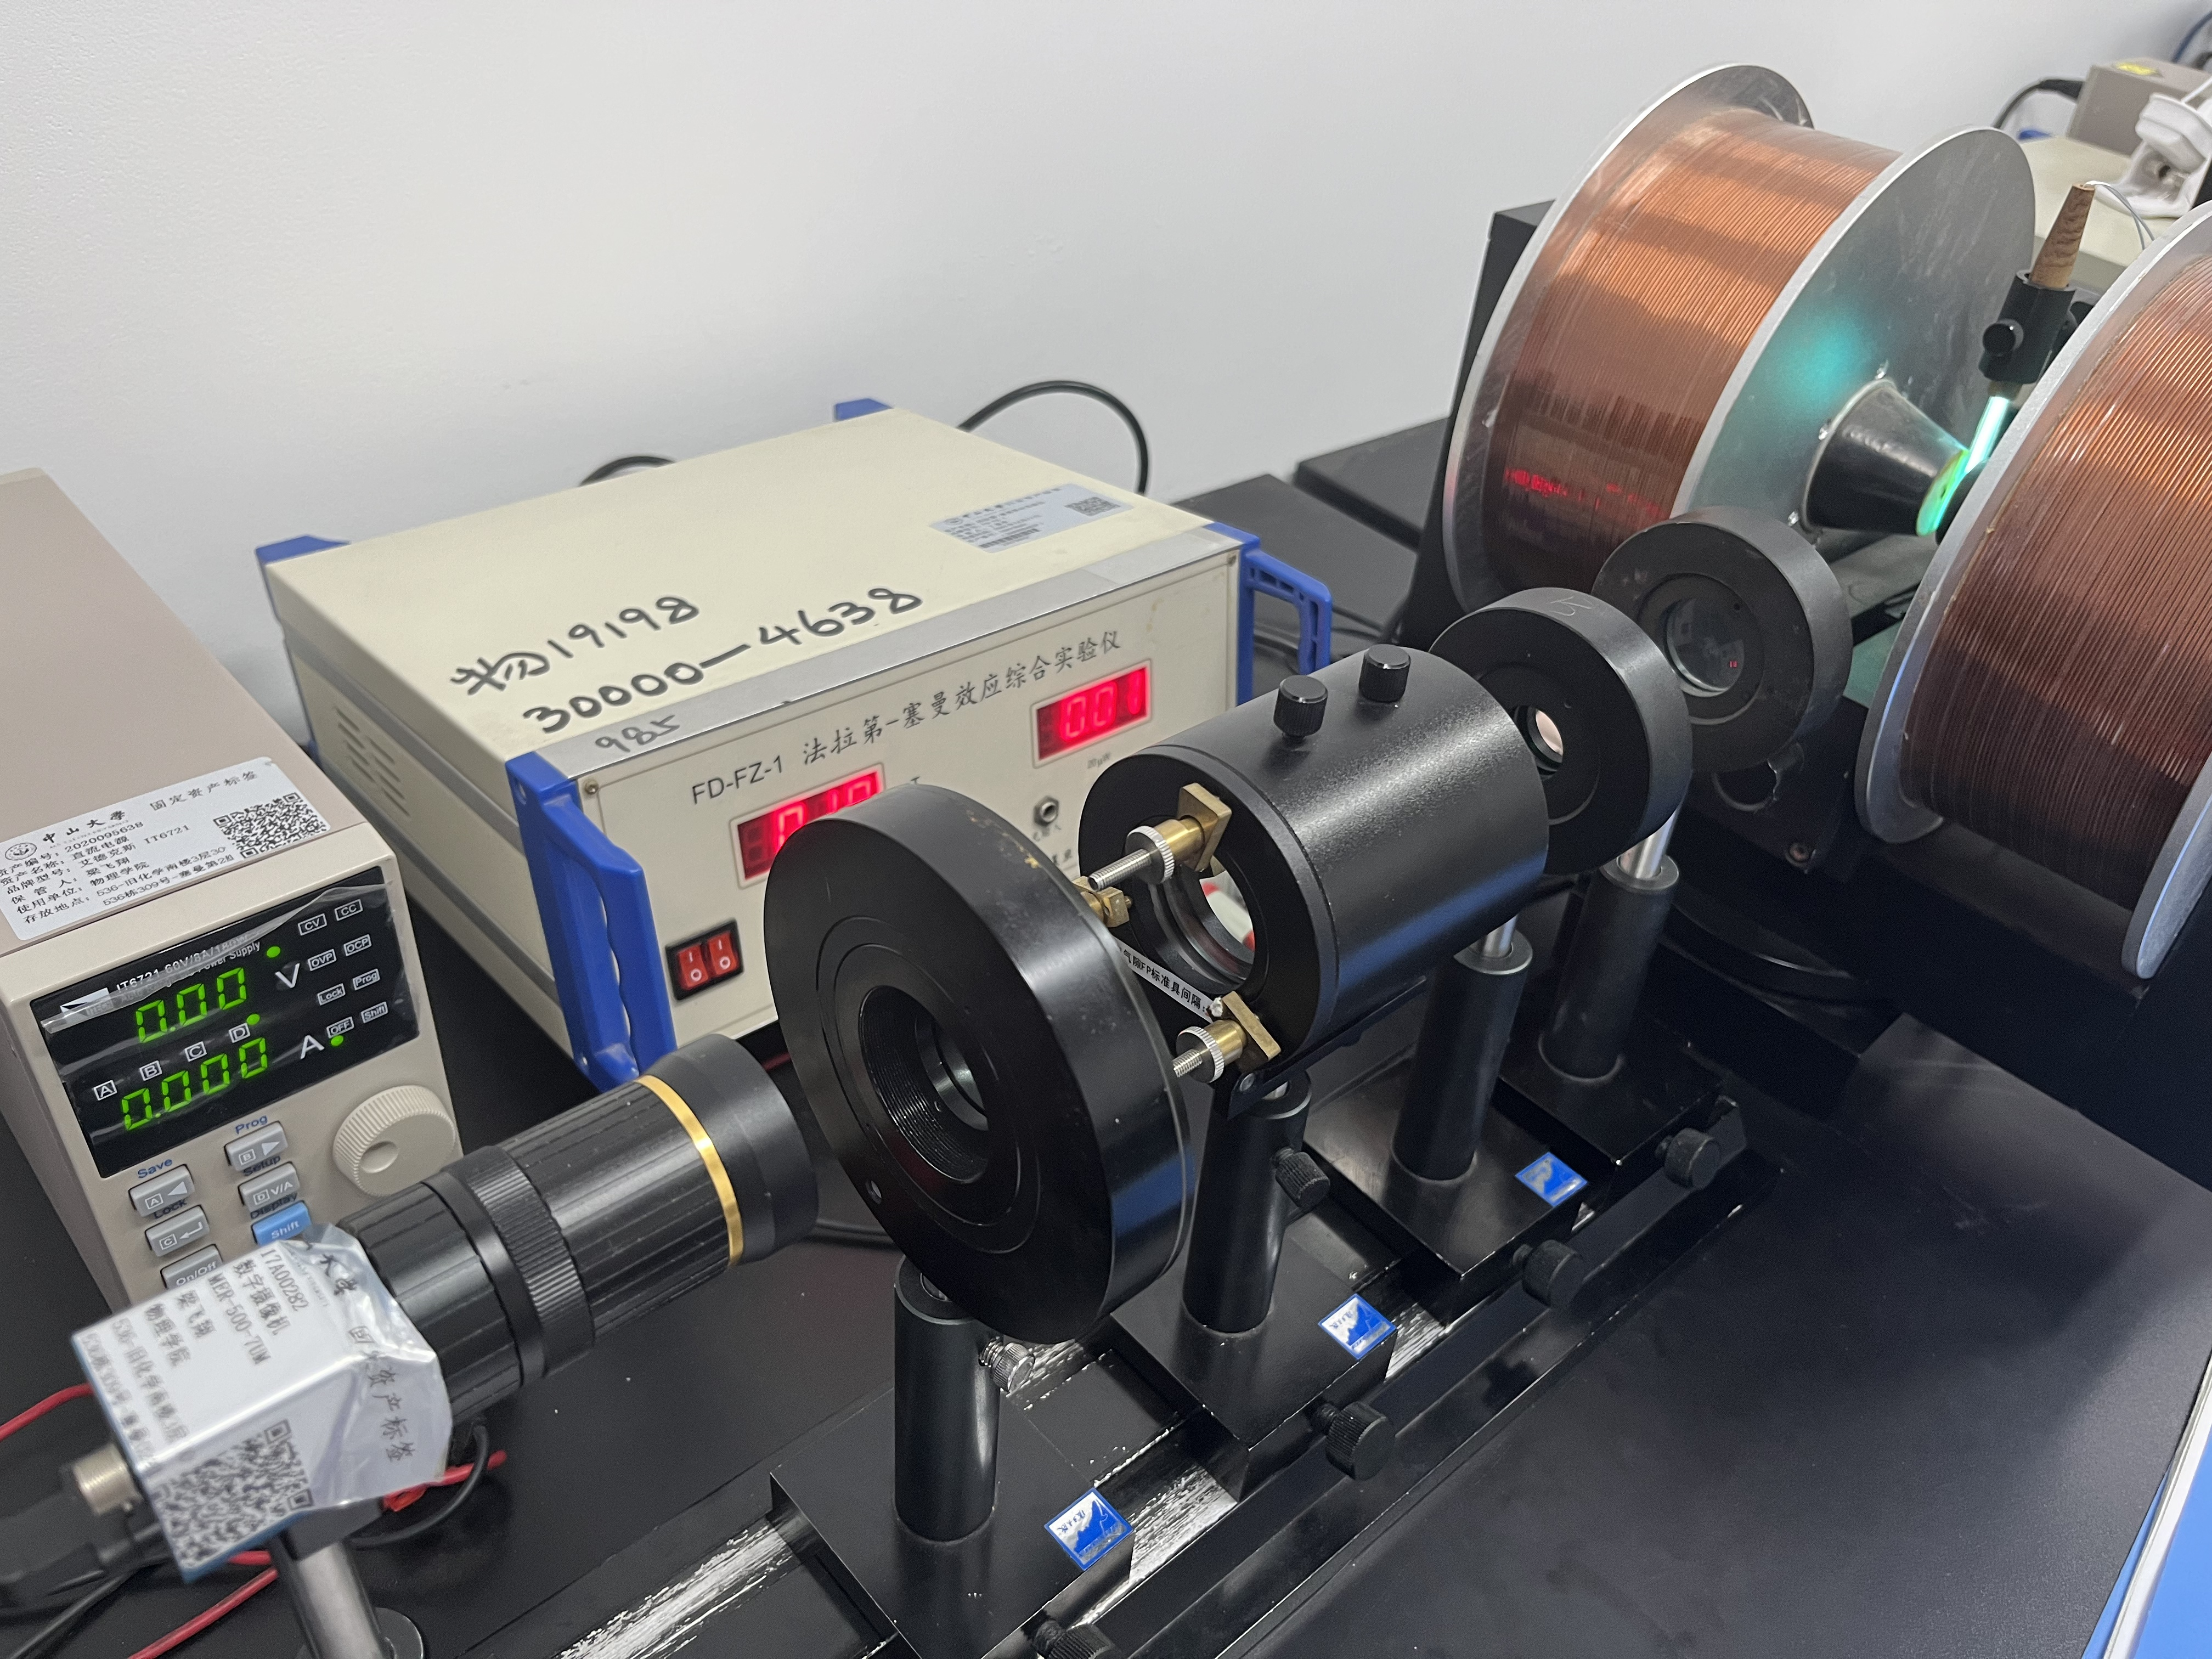
\includegraphics[width=0.8\textwidth]{实物光路.jpg}
    \caption{塞曼效应实验光路实物图}
    \label{fig:setup}
\end{figure}

调节后我们可以观察到第一周实验中相似的现象，如图\ref{fig:Zeeman}所示，在此基础上开始第二周的实验。

\begin{figure}[h!]
    \centering
    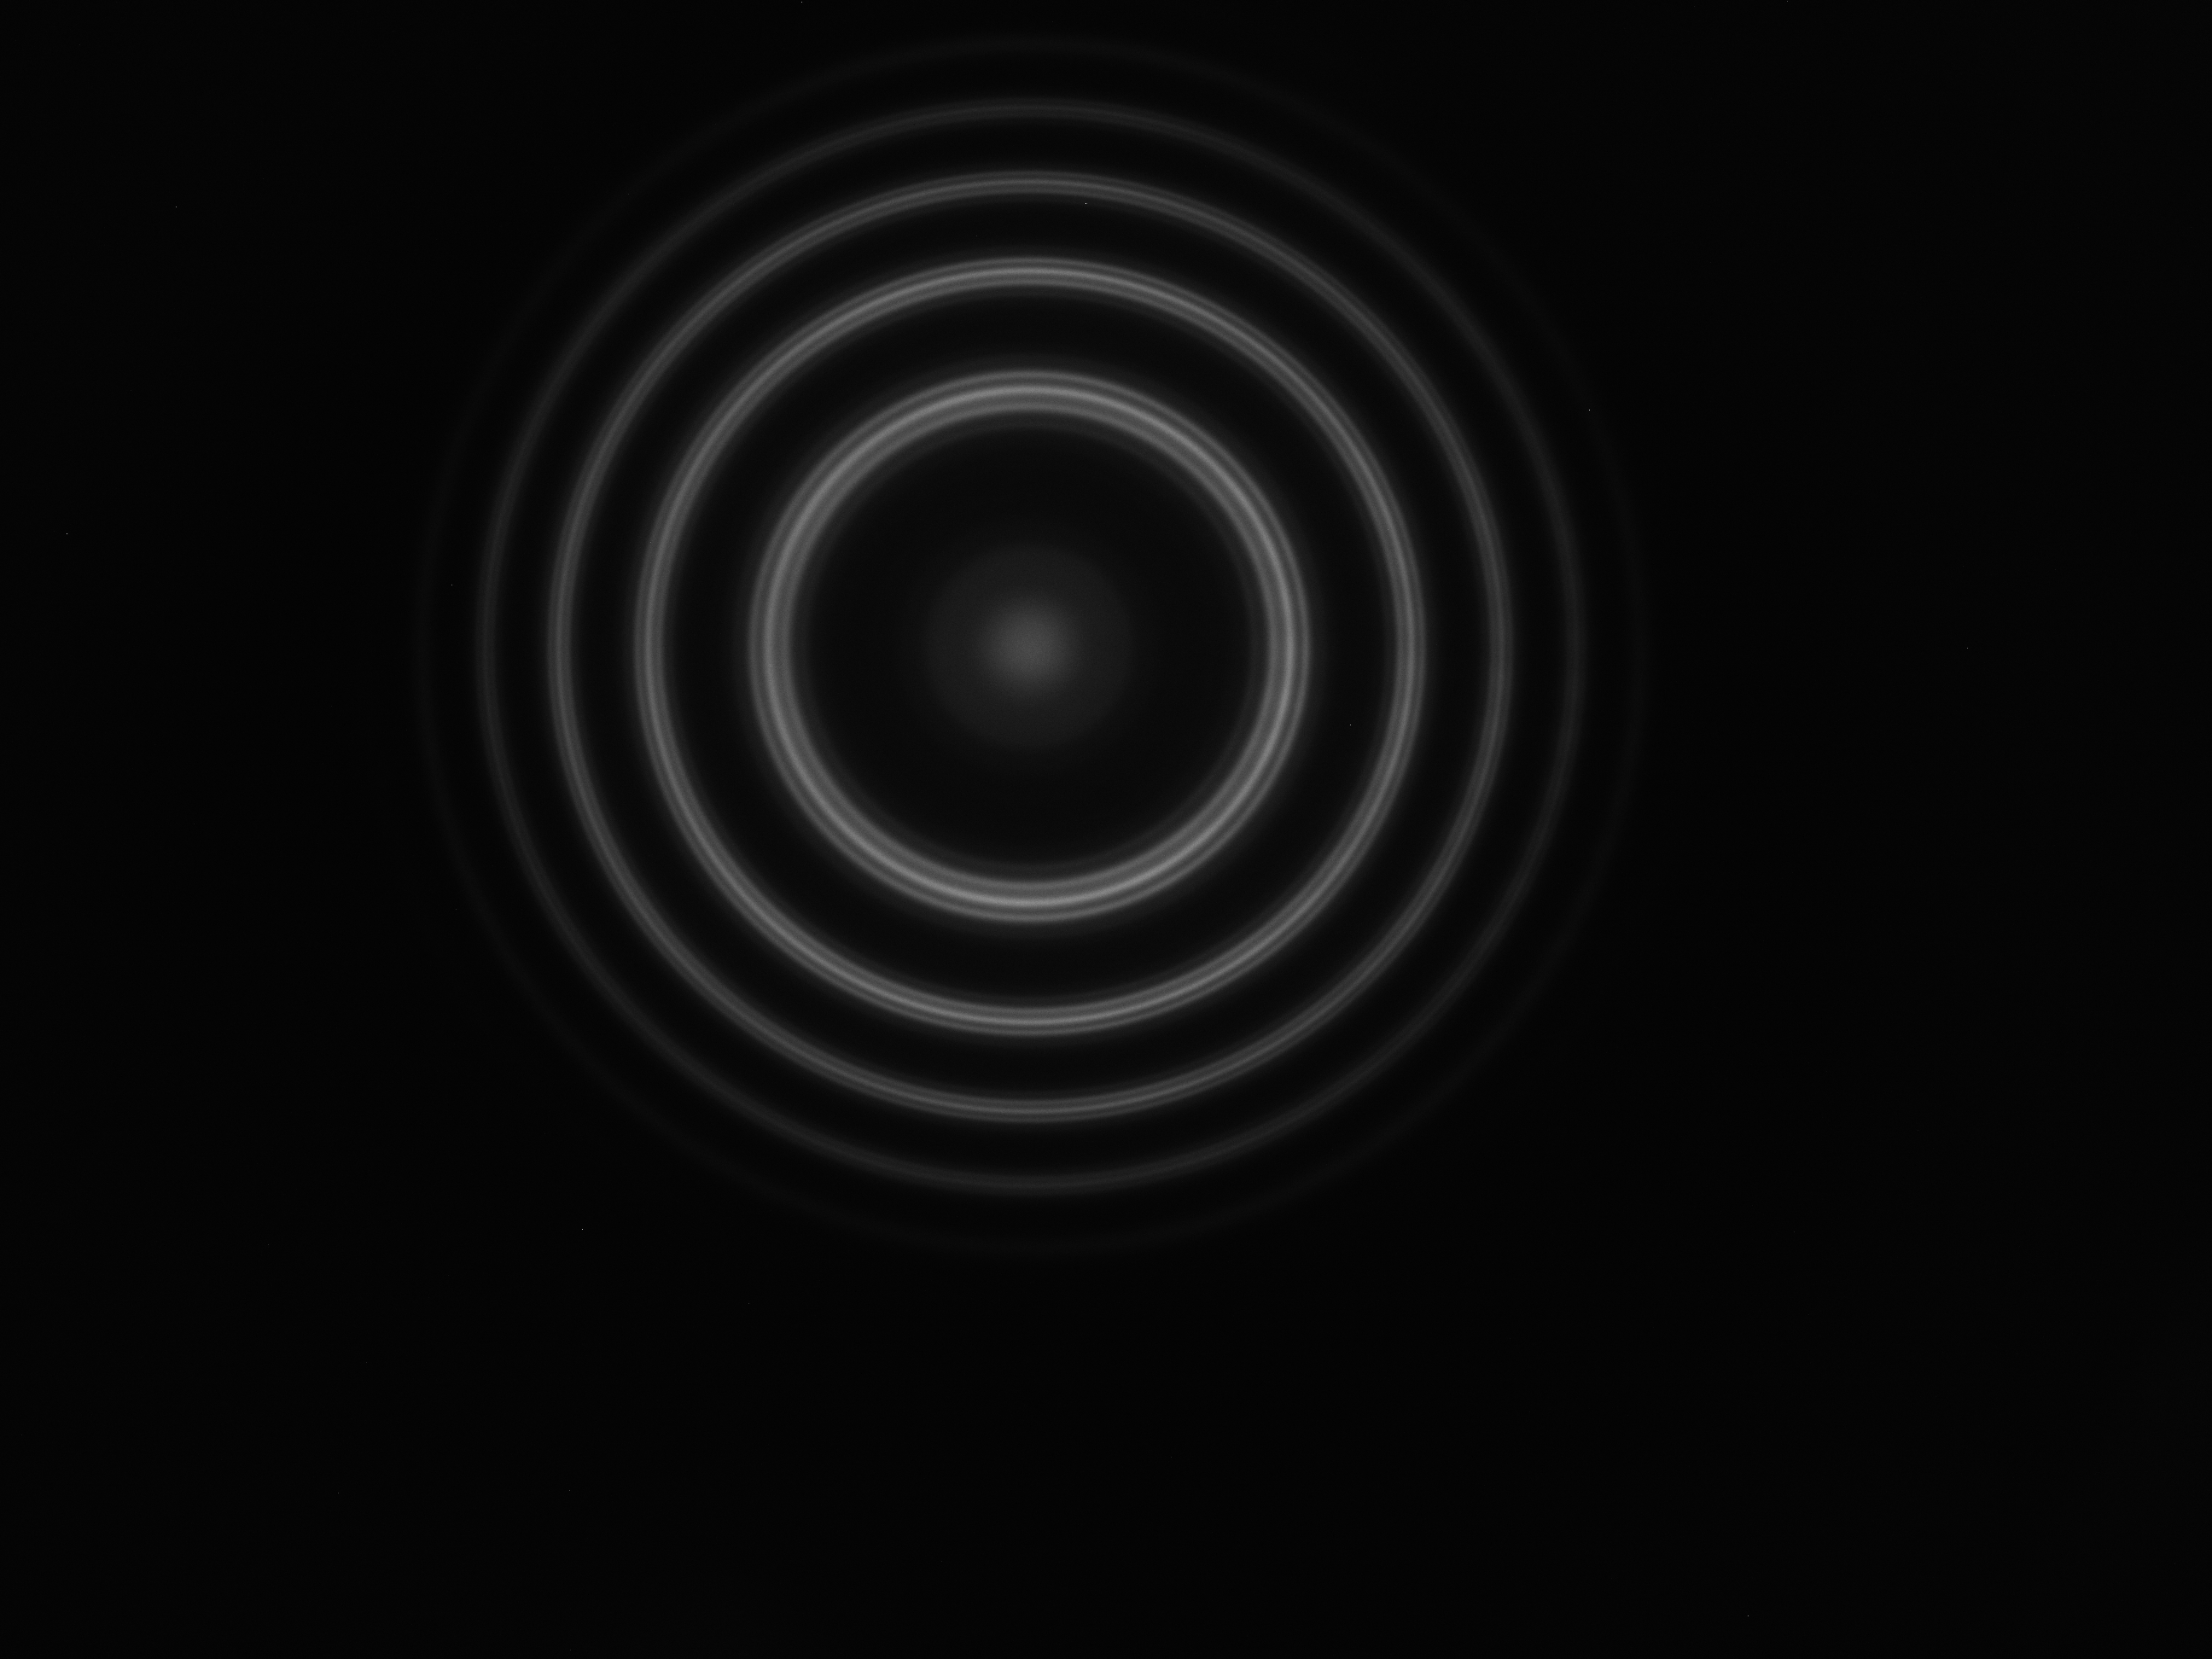
\includegraphics[width=0.8\textwidth]{调节.png}
    \caption{塞曼效应谱线分裂现象}
    \label{fig:Zeeman}
\end{figure}

随后为了观察正常塞曼效应$579.06\mathrm{nm}$的谱线，我们需要更换光路中的滤波片，使得对应的正常塞曼效应的谱线能够清晰地显示在CCD上。
由于滤波片的带通范围内还有一条波长略小于$579.06\mathrm{nm}$的谱线，因此我们需要稍微调整滤波片的角度，使得带通范围略有增大，这样便能只观察这一条谱线。
结果如图\ref{fig:filter1}和\ref{fig:filter2}所示。

\begin{figure}[h!]
    \centering
    \begin{minipage}[t]{0.48\textwidth}
        \centering
        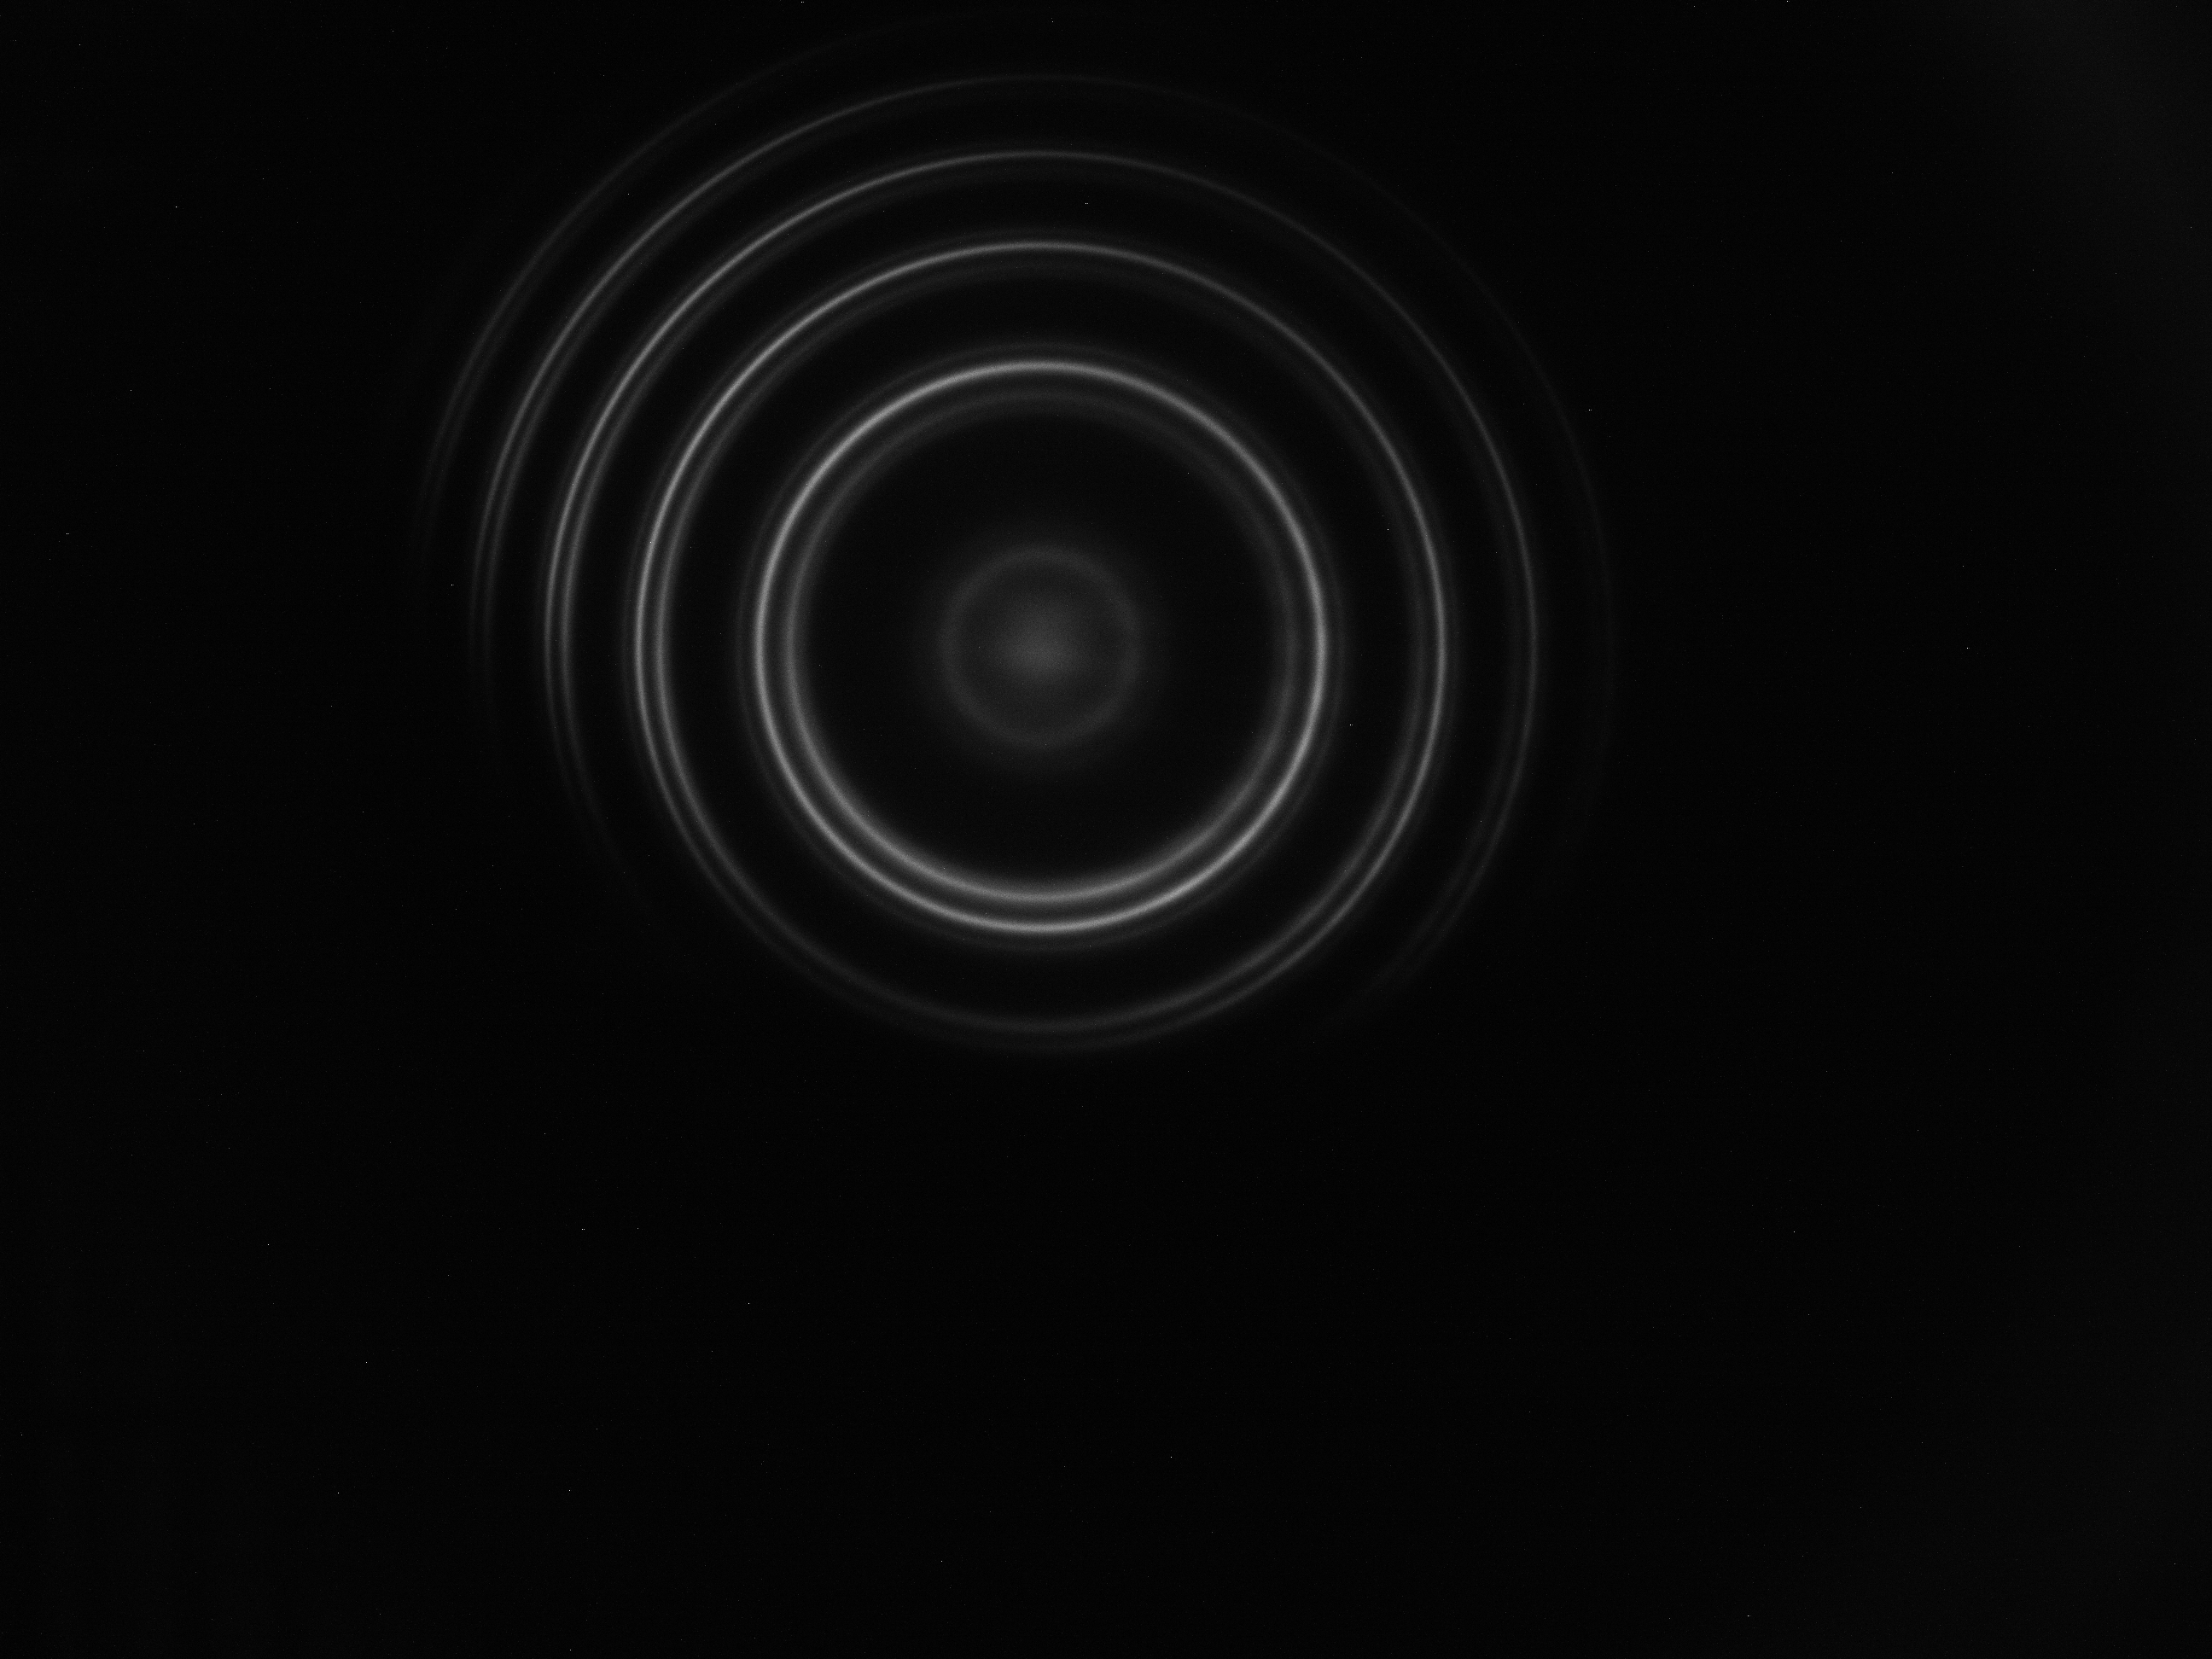
\includegraphics[width=\textwidth]{!2.png}
        \caption{可见两条谱线}
        \label{fig:filter1}
    \end{minipage}
    \hfill
    \begin{minipage}[t]{0.48\textwidth}
        \centering
        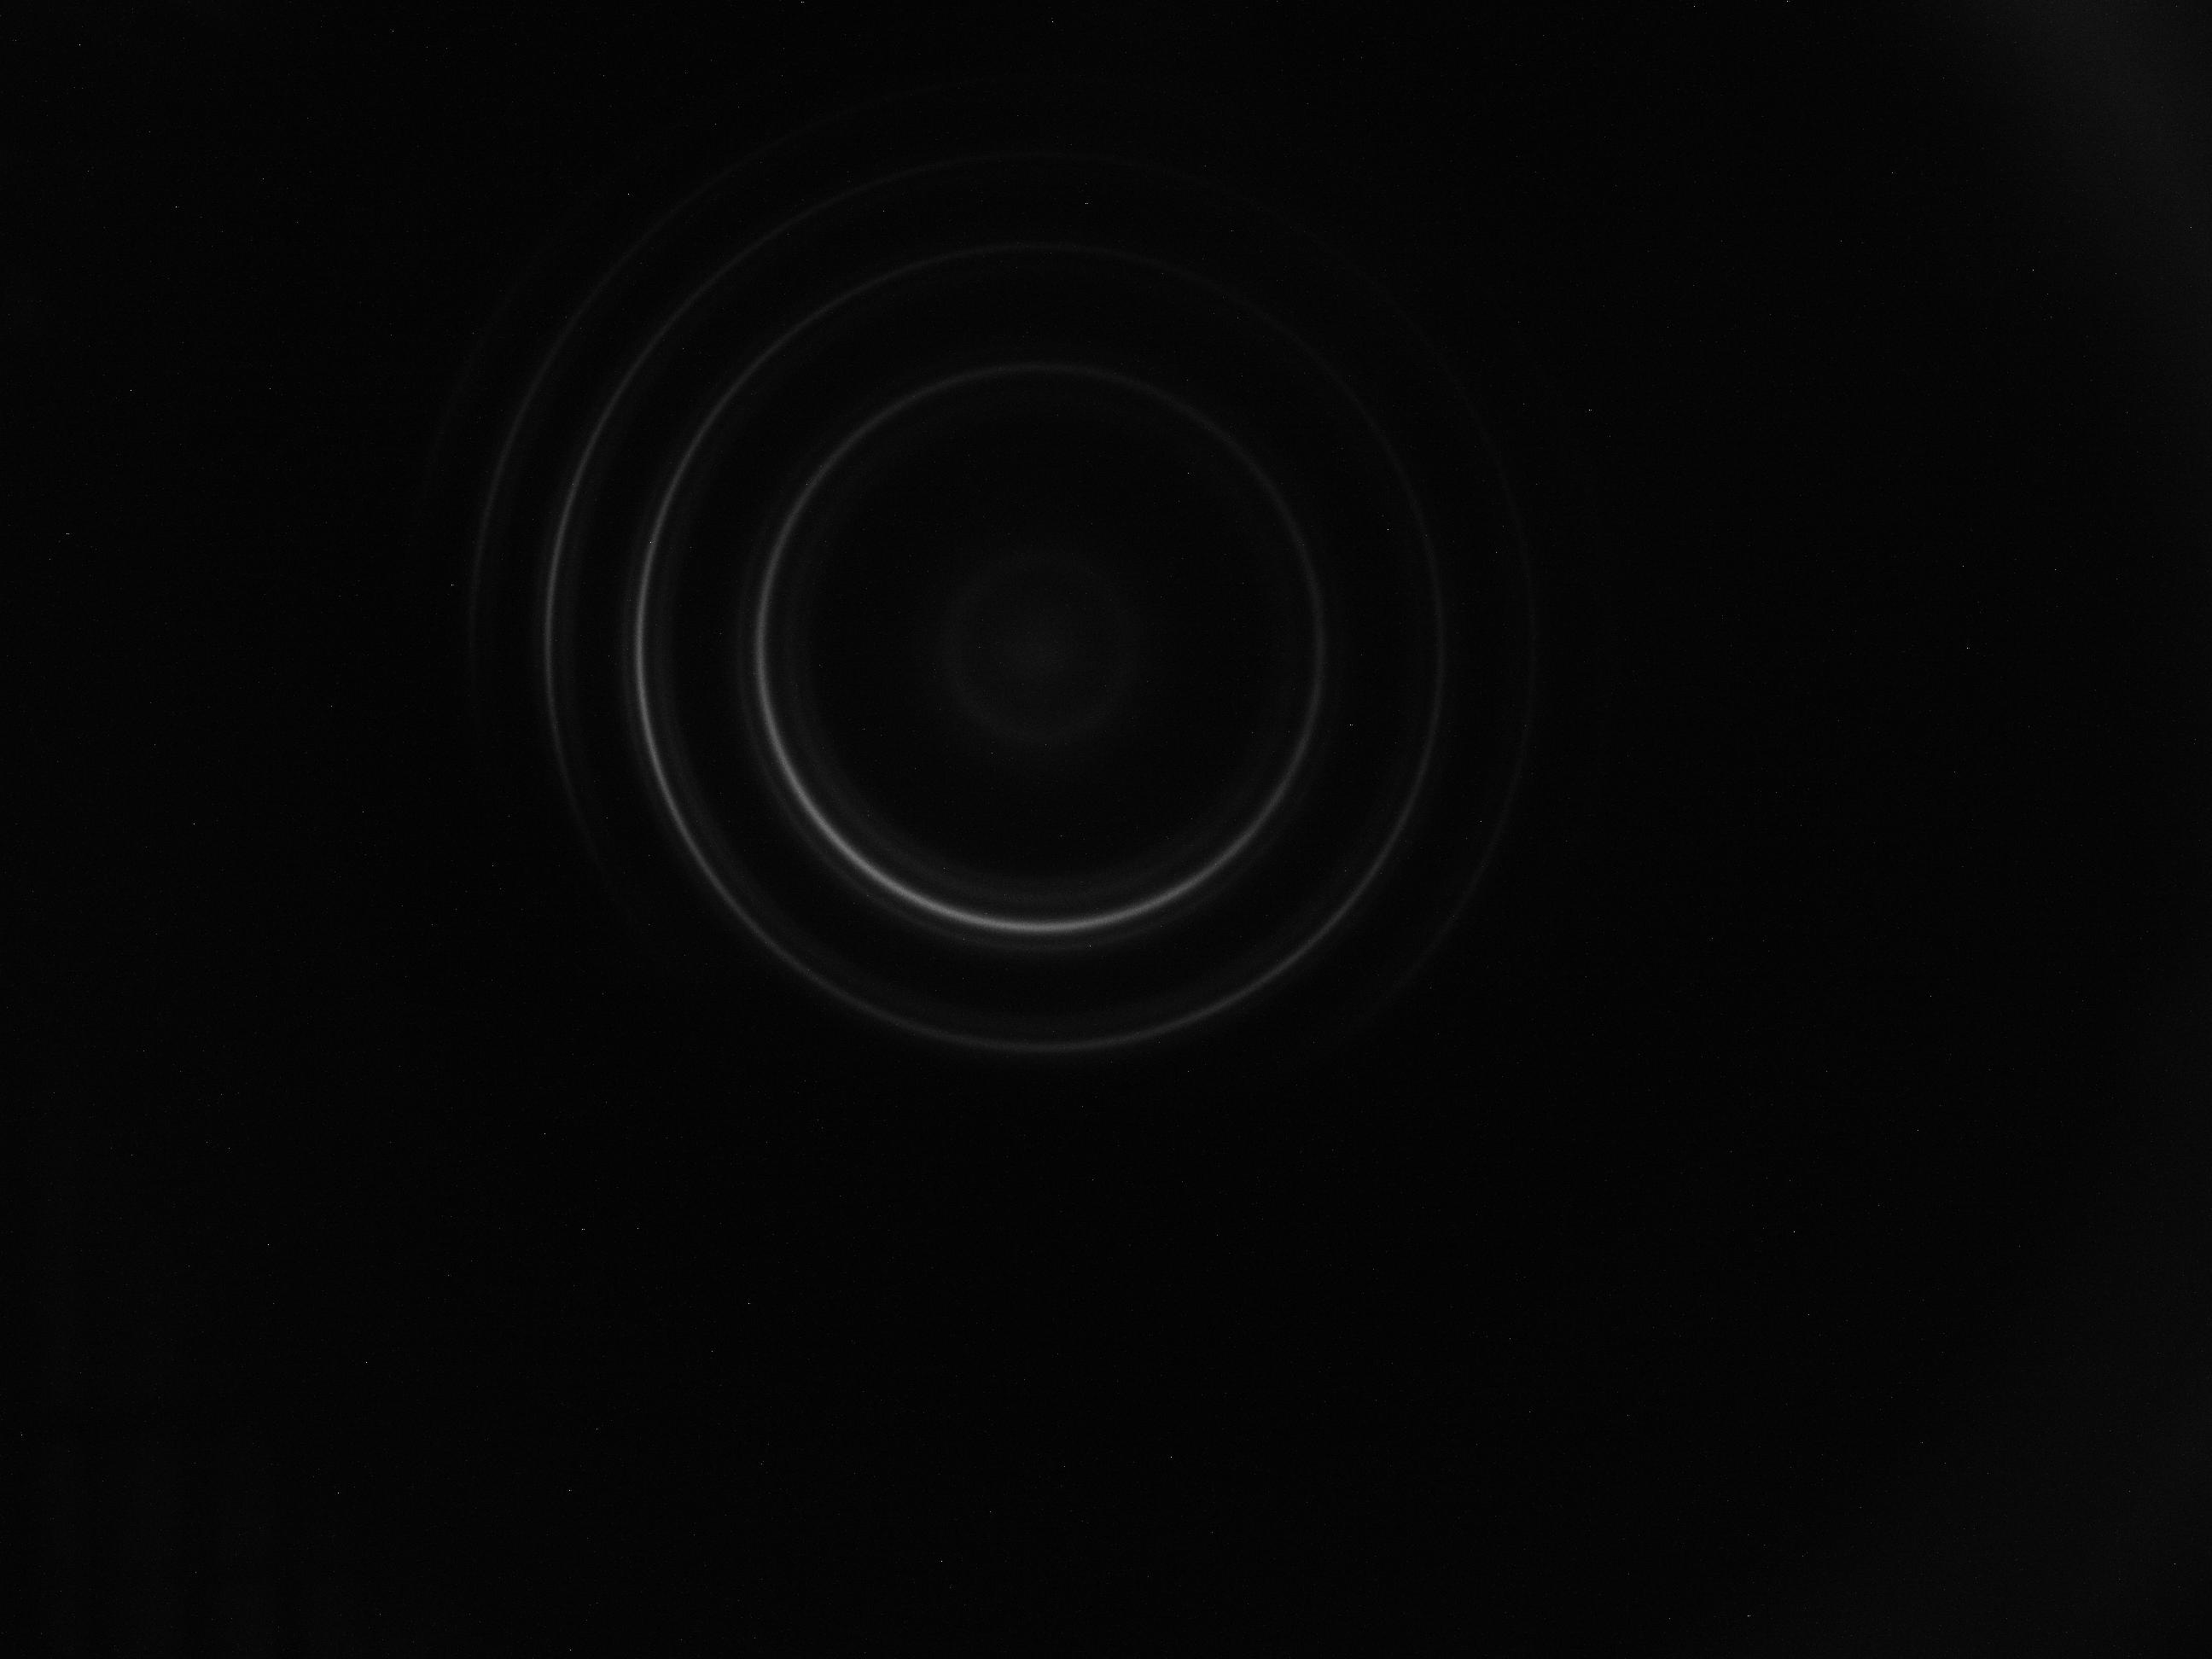
\includegraphics[width=\textwidth]{579.07.jpg}
        \caption{$579.07\mathrm{nm}$谱线}
        \label{fig:filter2}
    \end{minipage}
\end{figure}

\subsubsection*{磁场标定}
由于两周实验间隔较长，且我们重新调节了光路，有可能汞灯所在的位置发生了变化，因此我们需要重新标定磁场。
具体的过程和操作均与第一周实验相同，这里不再详细赘述，原始数据可以在文末原始数据记录的部分找到。

\subsubsection*{观察正常塞曼效应}
和上周的实验步骤相似，我们在不同励磁电流大小下观察正常塞曼效应的谱线分裂情况，结果如图\ref{fig:Zeeman_normal1}、\ref{fig:Zeeman_normal2}和\ref{fig:Zeeman_normal3}所示。

\begin{figure}[h!]
    \centering
    \begin{minipage}[t]{0.48\textwidth}
        \centering
        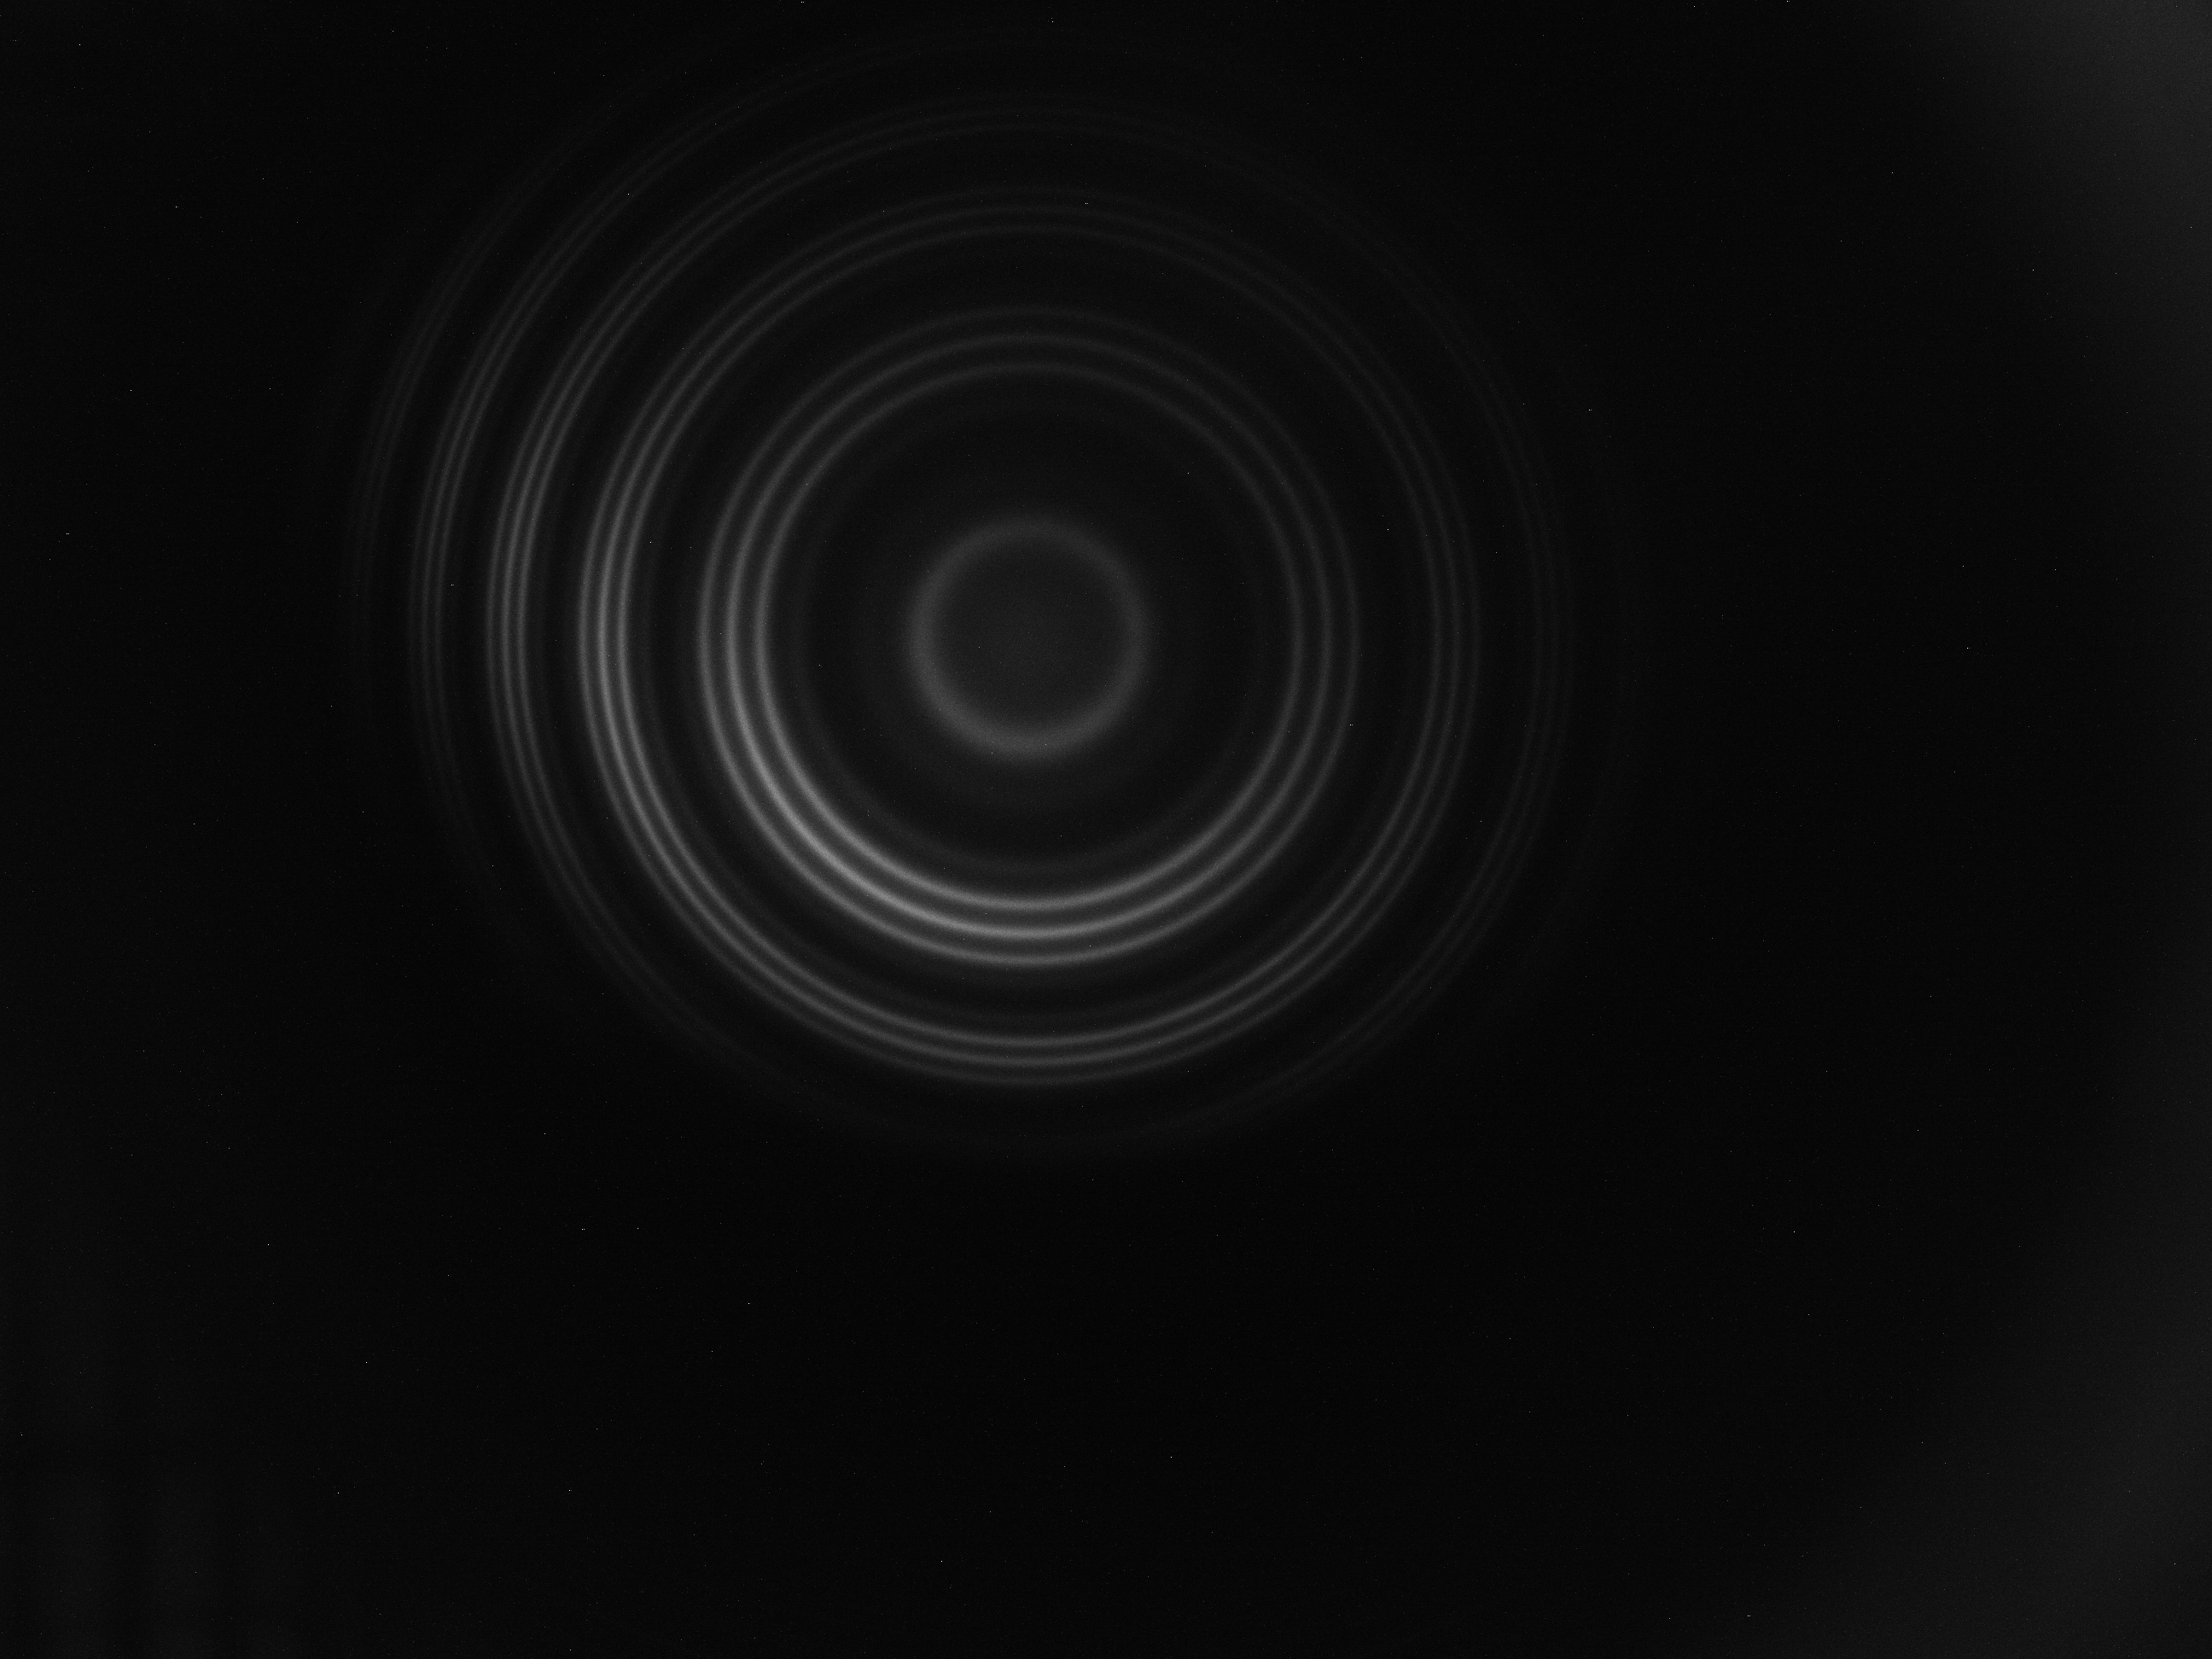
\includegraphics[width=\textwidth]{B=3.png}
        \caption{I=3A}
        \label{fig:Zeeman_normal1}
    \end{minipage}
    \hfill
    \begin{minipage}[t]{0.48\textwidth}
        \centering
        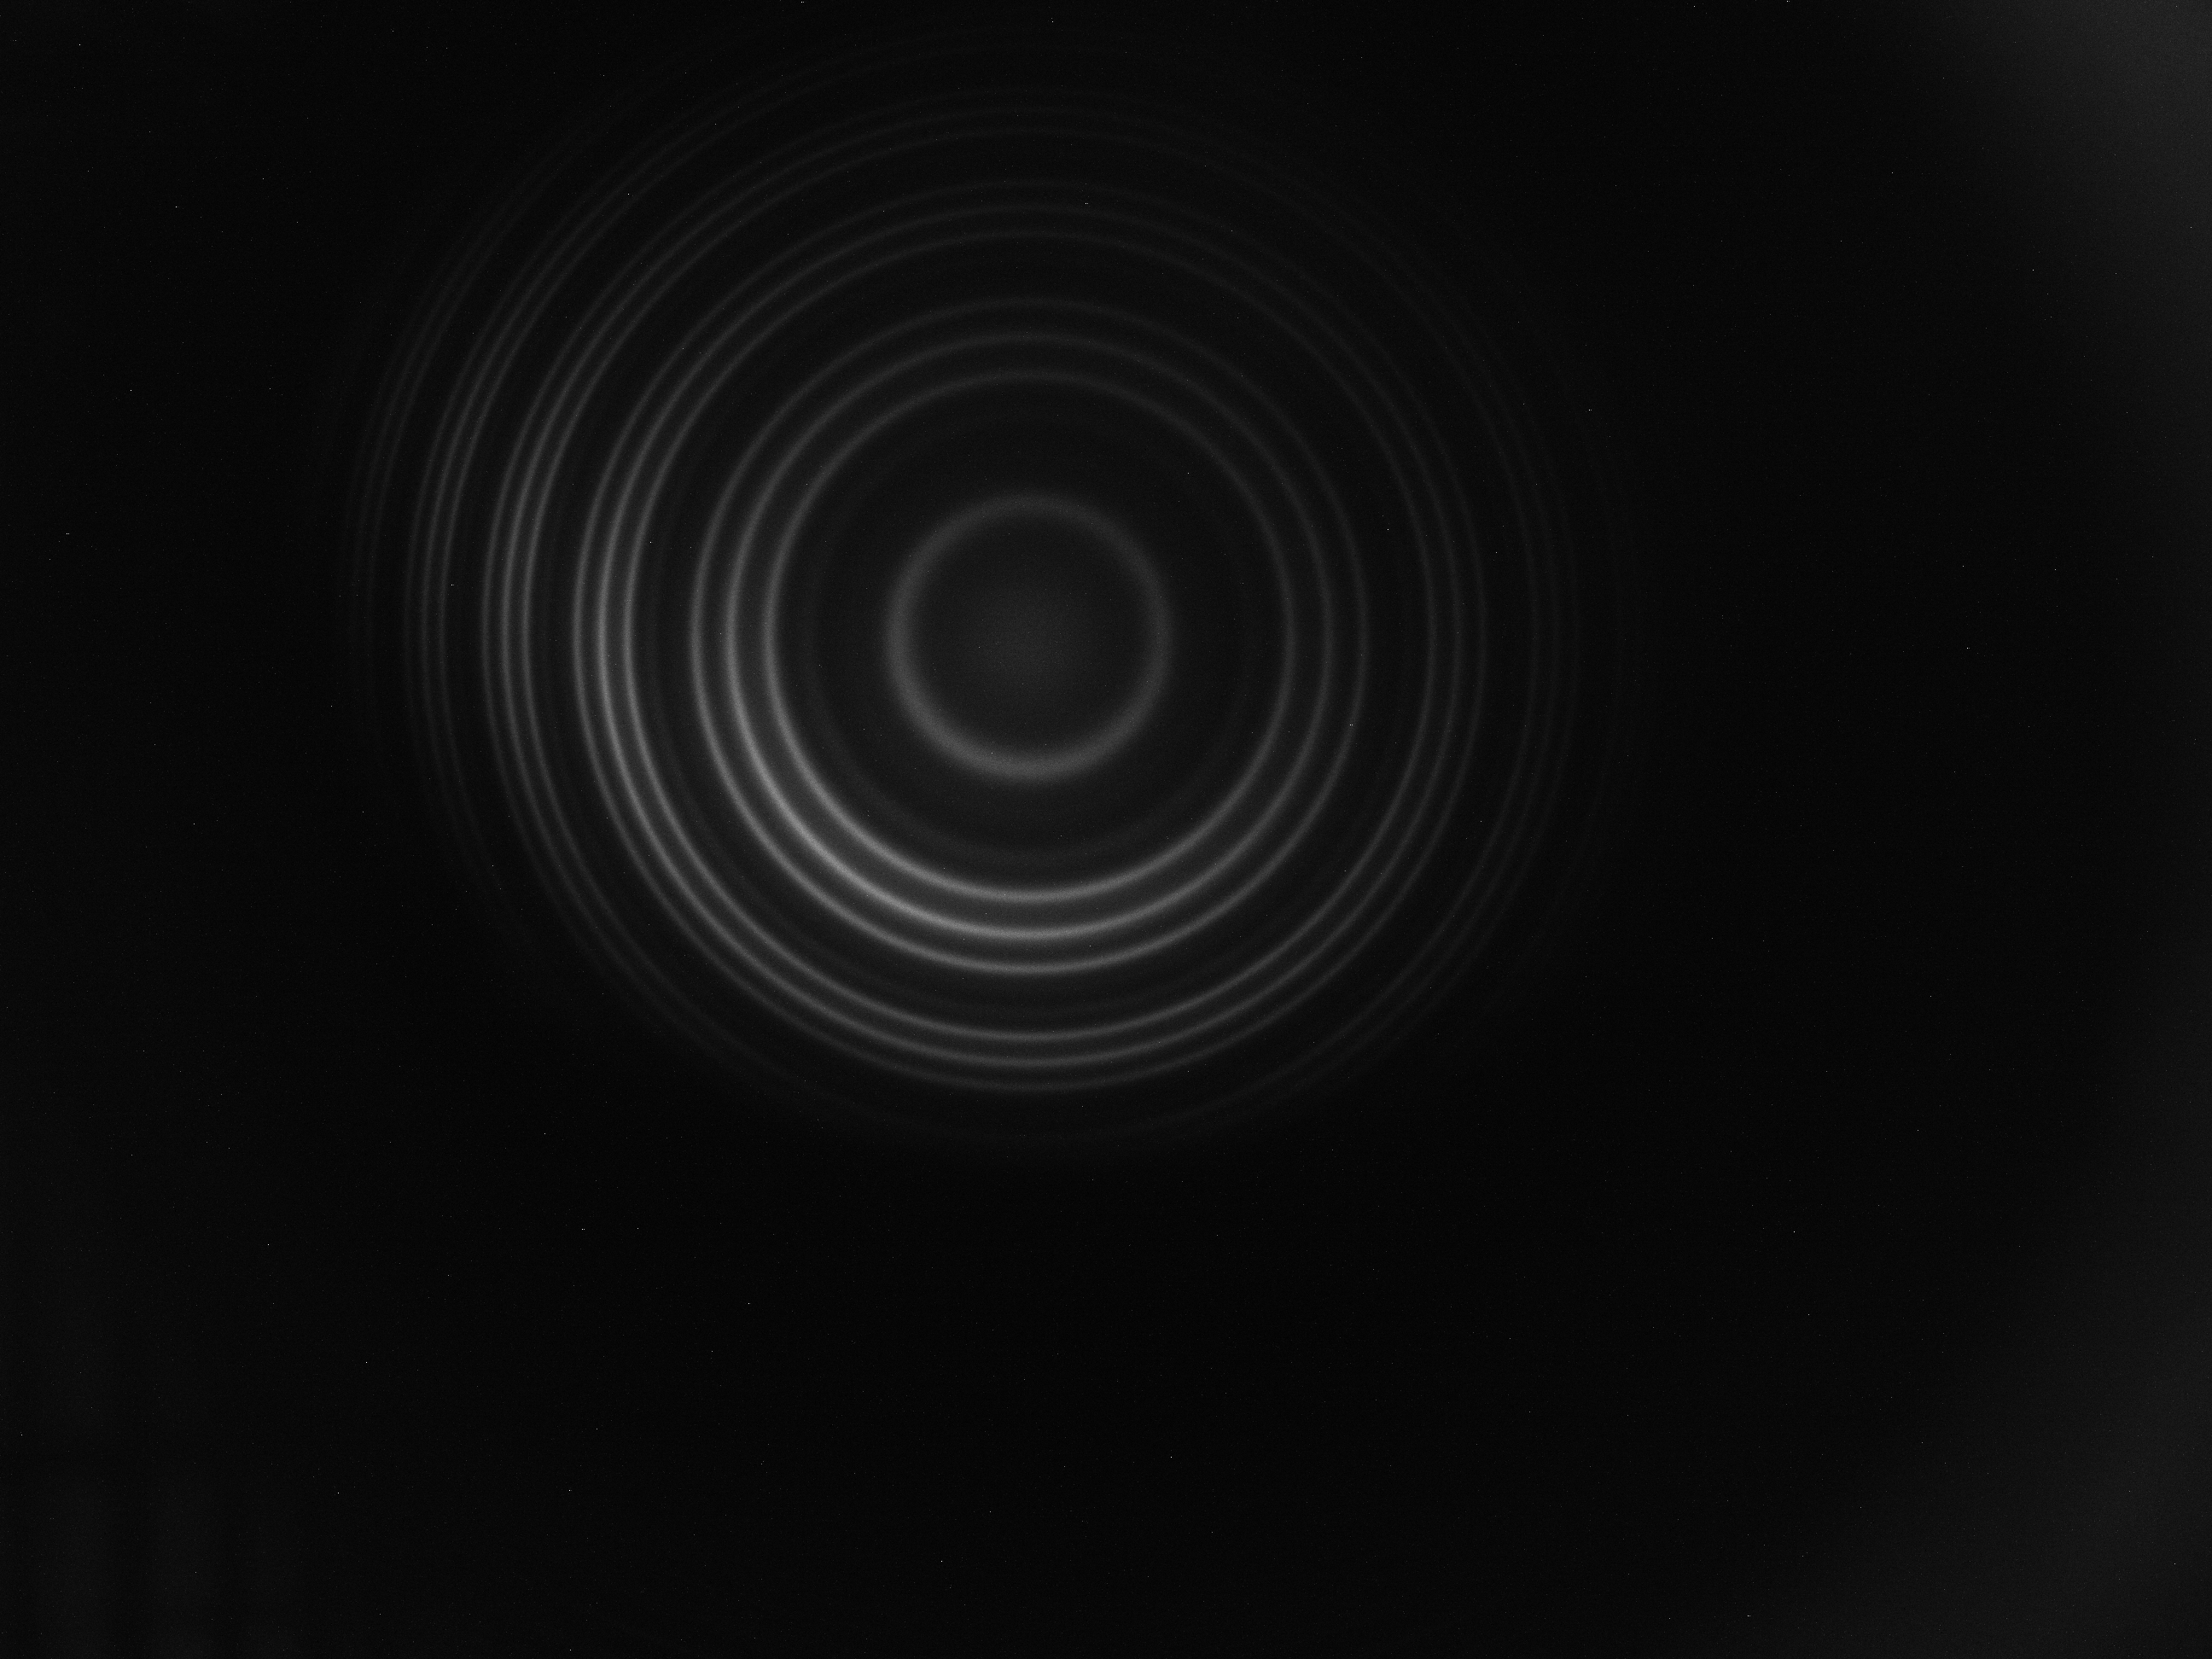
\includegraphics[width=\textwidth]{B=4.png}
        \caption{I=4A}
        \label{fig:Zeeman_normal2}
    \end{minipage}
\end{figure}

\begin{figure}[h!]
    \centering
    \begin{minipage}[t]{0.48\textwidth}
        \centering
        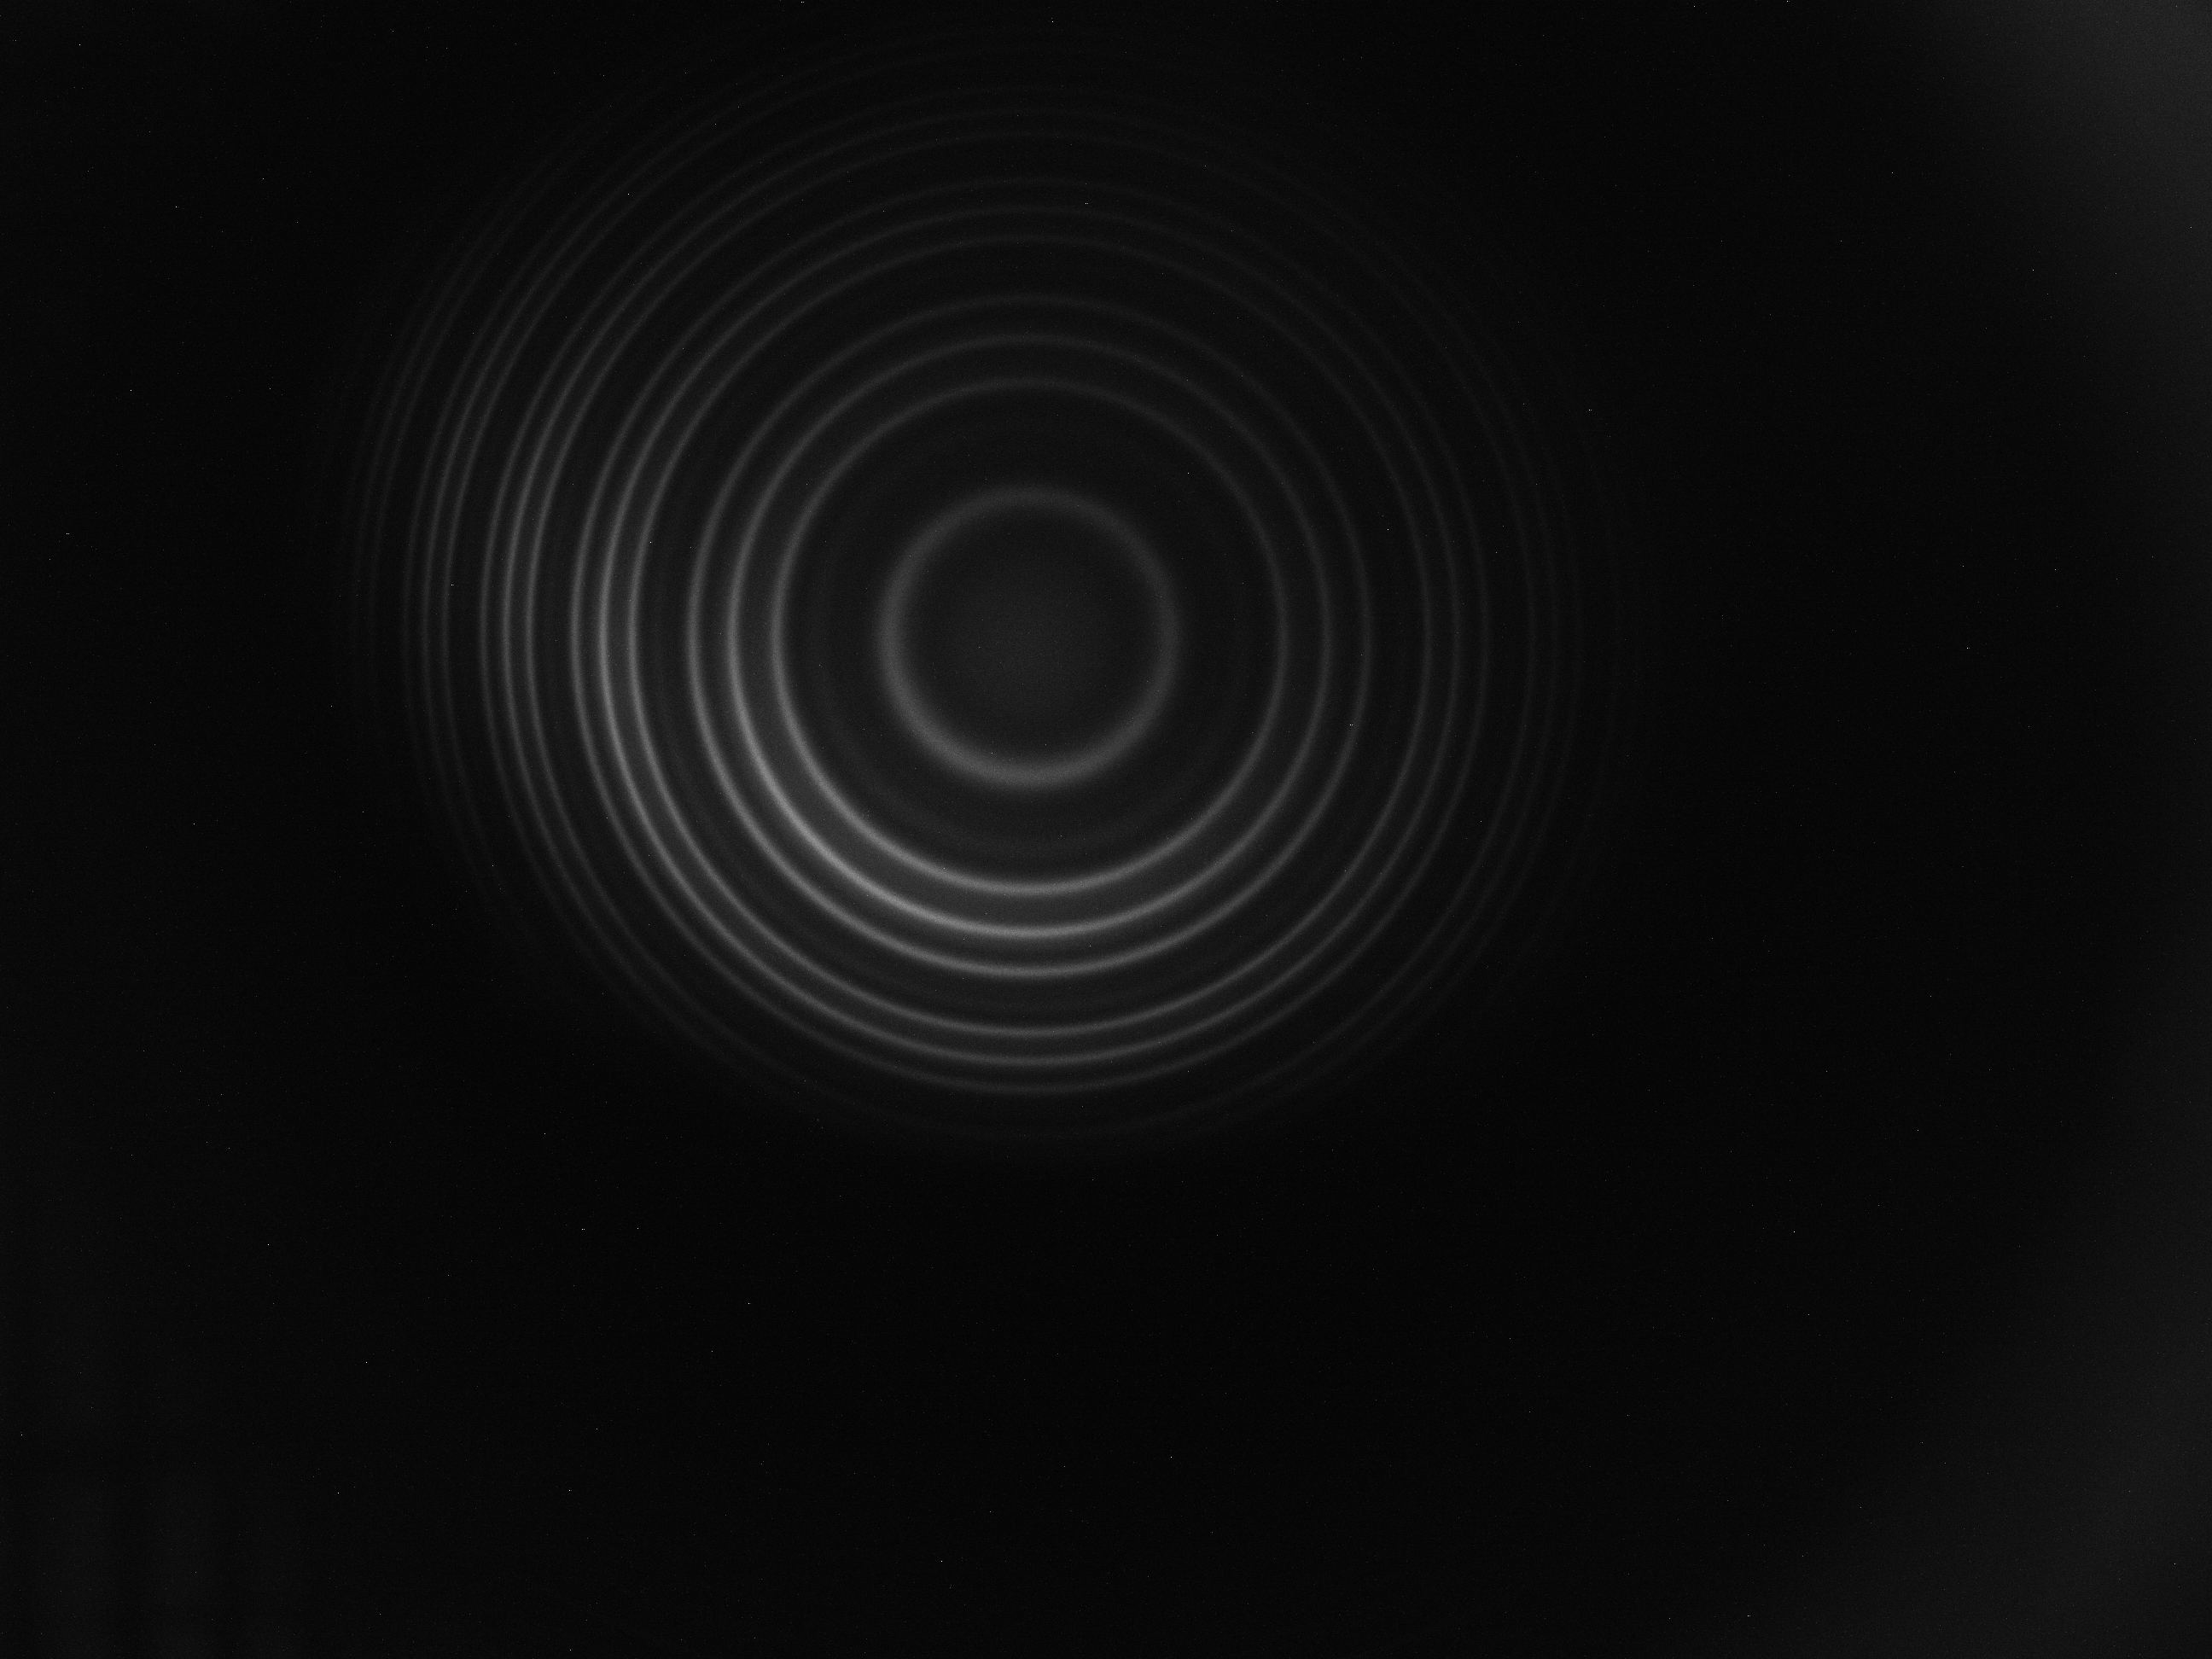
\includegraphics[width=\textwidth]{B=5.png}
        \caption{I=5A}
        \label{fig:Zeeman_normal3}
    \end{minipage}
\end{figure}

\subsubsection*{利用正常塞曼效应计算荷质比}
和上周的实验步骤相似，我们在不同励磁电流大小下观察正常塞曼效应的谱线分裂情况，结果如图\ref{fig:Zeeman_normal1}、\ref{fig:Zeeman_normal2}和\ref{fig:Zeeman_normal3}所示。
计算公式为
\begin{equation}
  \frac{e}{m} = \frac{2\pi c}{d \, B} \, \frac{D_{b}^{2}-D_{a}^{2}}{D_{N-1}^{2}-D_{N}^{2}}
\end{equation}

\begin{table}[h!]
  \centering
  \begin{tabular}{|c|c|c|c|c|c|c|}
      \hline
      电流(A) & 磁场(mT) & $D_a / D_N$(pix) & $D_b$(pix) & $D_{N-1}$(pix)  & $\cfrac{e}{m}(10^{11}\mathrm{C/kg})$ & 相对误差($\%$) \\
      \hline\hline
      4.019 & 992.7 & 329 & 289 & 478 & 1.805 & $2.7\%$ \\
      4.509 & 1081.3& 328 & 288 & 479 & 1.745 & $0.8\%$ \\
      3.009 & 771.2 & 327 & 296 & 478 & 1.792 & $1.9\%$ \\
      \hline
  \end{tabular}
  \caption{不同电流值下的测量数据}
  \label{tab:measurements_normal}
\end{table}

这个误差依然是在$2\%$左右，符合实验要求。

\subsubsection*{误差分析}
在本次实验中，我们测量得到的荷质比与理论值的相对误差在$1.5\%$左右，这个误差主要来源于以下几个方面：

\begin{enumerate}
  \item \textbf{磁场测量误差}：
  \begin{itemize}
      \item 磁场探头的位置与汞灯光源位置存在偏差，导致实际作用于原子的磁场强度与测量值存在差异
      \item 电流-磁场关系曲线拟合过程中可能存在系统误差
      \item 汞灯在测量过程中可能存在微小位移，影响测量精度
  \end{itemize}

  \item \textbf{光路调节误差}：虽然我们反复调节了光路中各元件的位置，但可能并未达到最佳状态。F-P标准具的平行度、光轴的对准程度等都会影响干涉条纹的清晰度和对称性，从而影响测量精度。
    
  \item \textbf{CCD成像误差}：
  \begin{itemize}
    \item 对焦不够清晰导致谱线边缘模糊，增加了确定谱线位置的难度
    \item 手动设置干涉条纹中心位置时，由于缺乏精确的参考点，可能存在几个像素的偏差
  \end{itemize}
    
  \item \textbf{测量操作误差}：使用鼠标光标测量圆环半径时，由于人眼判断和鼠标操作的限制，可能存在3-4个像素的误差
\end{enumerate}

为了减小这些误差，我们可以在后续实验中：

\begin{itemize}
    \item 更仔细地调节光路，确保F-P标准具的平行度和光轴对准
    \item 使用更高分辨率的CCD相机，提高图像清晰度
    \item 开发自动化的图像处理程序，减少人为操作误差
    \item 改进磁场测量方法，确保探头位置与光源位置一致
\end{itemize}

\subsection*{【思考题】}

\subsubsection*{1. 随磁场强度增大，横向/纵向塞曼效应谱线裂分数量与裂距的变化规律}

\paragraph{裂分数量}  
对于给定的原子能级，其总角动量量子数为 $J$，在外加磁场 $B$ 下，该能级会分裂为 $2J+1$ 个子能级，磁量子数 $M$ 取值为
\[
M = -J,\ -J+1,\ \dots,\ +J\,.
\]
发生跃迁时，需满足选择定则 $\Delta M = 0, \pm 1$。因此，若上能级和下能级的 $J$ 值分别为 $J_2$ 与 $J_1$，则总的可能谱线数目为满足
\[
M_2 - M_1 = 0, \pm 1
\]
的所有组合数。  
\begin{itemize}
  \item 当 $g_2 = g_1 = 1$（朗德因子相等）时，分裂为三条谱线（正常塞曼效应）。  
  \item 当 $g_2 \neq g_1$ 时，分裂条数可能超过三条（反常塞曼效应），其具体条数由所有可能的 $(M_2,\,M_1)$ 对确定。  
\end{itemize}
\paragraph{裂距变化}  
在弱磁场区间（Zeeman 区），裂距 $\Delta E$ 与磁场强度 $B$ 呈线性关系：
\[
\Delta E = g\,\mu_B\,B\,\Delta M \,,
\qquad \mu_B = \frac{e\hbar}{2m}\,,
\]
对应的波长偏移 $\Delta \lambda$ 满足
\[
\Delta E = \frac{hc}{\lambda^2}\,\Delta \lambda \quad\Longrightarrow\quad \Delta \lambda = \frac{\lambda^2}{hc}\,g\,\mu_B\,B\,\Delta M \,.
\]
因此，随着 $B$ 增大，谱线 $\pi$ 和 $\sigma^\pm$ 分量的间距（波长或波数）也按照上述线性关系增大。在横向观察（观察方向垂直于 $B$）时，可看到中心的 $\pi$ 线和对称分布的两条 $\sigma^\pm$ 线，其距离随 $B$ 增大而增大；在纵向观察（观察方向平行于 $B$）时，仅能观测到 $\sigma^\pm$ 线，同样其间距随 $B$ 增大线性增大。  

当磁场强度进一步增大到足以破坏轨道–自旋耦合耦合能，进入 Paschen–Back 区域时，能级分裂趋于简化，理论上近似回到线性三线模式，但此时 $g$ 值近似为轨道贡献或自旋贡献的简单叠加，且不再与原先的 LS 耦合朗德因子严格相同。

\subsubsection*{2. F–P 标准具的自由光谱范围、精细度及最小可分辨波长差}

已知条件：
\[
d = 2\,\text{mm} = 2.0 \times 10^{-3}\,\text{m}, 
\quad R = 95\% = 0.95, 
\quad \lambda = 500\,\text{nm} = 5.0 \times 10^{-7}\,\text{m}.
\]

\paragraph{(1) 自由光谱范围 $\Delta \lambda_F$}  
Fabry–Pérot 标准具的自由光谱范围定义为相邻两条同级条纹所能分辨的最大波长差，即
\[
\Delta \lambda_F = \frac{\lambda^2}{2d}\,.
\]
代入数值：
\[
\Delta \lambda_F \;=\; \frac{(5.0 \times 10^{-7}\,\mathrm{m})^2}{2 \times 2.0 \times 10^{-3}\,\mathrm{m}}
\;=\; \frac{25.0 \times 10^{-14}}{4.0 \times 10^{-3}}
\;=\; 6.25 \times 10^{-11}\,\mathrm{m}
\;=\; 0.0625\,\mathrm{pm}\,.
\]

\paragraph{(2) 精细度 $F$}  
精细度定义为
\[
F = \frac{\pi \sqrt{R}}{1 - R} \,.
\]
代入 $R = 0.95$，有
\[
\sqrt{R} = \sqrt{0.95} \approx 0.9747, 
\quad
1 - R = 0.05,
\]
\[
F \;=\; \frac{\pi \times 0.9747}{0.05} 
\;\approx\; \frac{3.061}{0.05} 
\;\approx\; 61.22\,.
\]

\paragraph{(3) 最小可分辨波长差 $(\delta \lambda)_{\min}$}  
最小可分辨波长差近似由
\[
(\delta \lambda)_{\min} = \frac{\Delta \lambda_F}{F}
\]
给出，于是
\[
(\delta \lambda)_{\min} \;=\; \frac{6.25 \times 10^{-11}\,\mathrm{m}}{61.22} 
\;\approx\; 1.02 \times 10^{-12}\,\mathrm{m} 
\;=\; 1.02\,\mathrm{pm}\,.
\]
因此，在上述条件下，该 F–P 标准具的自由光谱范围约为 $0.0625\,\mathrm{pm}$，精细度约为 $61.2$，最小可分辨波长差约为 $1.02\,\mathrm{pm}$。

\subsubsection*{3. 由塞曼效应实验测定原子能级 $J$、$g$ 因子的方法}

\paragraph{(1) 测定 $J$}  
\begin{itemize}
  \item 当原子某一能级的总角动量量子数为 $J$ 时，该能级在外加磁场下将分裂为 $2J+1$ 个子能级。  
  \item 通过对某一条谱线（对应某一特定跃迁）的分裂条数进行统计。例如，若观测到在弱磁场条件下分裂出 $N$ 条谱线（$\pi$ 和 $\sigma$ 线一同计数），则可根据
  \[
    N = \text{(上能级子能级数)} + \text{(下能级子能级数)} - (\text{满足选择定则的抵消条数})
  \]
  来推算 $J_1$ 与 $J_2$，最简单的情形为 $J_2 = 1$，$J_1 = 0$ 时可观察到 3 条谱线。  
  \item 若已知下能级 $J_1$，则可从观测到的总分裂条数倒推出上能级 $J_2$；若两者均未知，则需多个测量点（不同能级的谱线分裂）联合分析。  
\end{itemize}

\paragraph{(2) 测定朗德因子 $g$}  
\begin{itemize}
  \item 在弱磁场下，任一子能级的能量改变量：
  \[
    \Delta E = g\,\mu_B\,B\,M,
    \qquad \mu_B = \frac{e\hbar}{2m}\,,
  \]
  其中 $M$ 为磁量子数。对应的波长偏移 $\Delta \lambda$ 满足
  \[
    \Delta E = \frac{hc}{\lambda^2}\,\Delta \lambda 
    \quad\Longrightarrow\quad 
    \Delta \lambda = \frac{\lambda^2}{hc}\,g\,\mu_B\,B\,\Delta M\,.
  \]
  \item 实验中可测得不同 $\Delta M$ 所对应的谱线间距（或相邻两条 $\sigma$ 线的波长差 $\Delta \lambda$），同时测量相应时刻的磁场强度 $B$。将上述公式改写为
  \[
    g = \frac{hc}{\lambda^2\,\mu_B\,B}\,\frac{\Delta \lambda}{\Delta M}\,,
  \]
  代入测得的 $\Delta \lambda$、$B$ 以及已知常数，即可求出 $g$。  
  \item 若多组 $B$ 值与对应 $\Delta \lambda$ 测量点一致，则可对多个点进行线性拟合，提高精度：  
  \[
    \Delta \lambda = \left( \frac{\lambda^2\,\mu_B}{hc} \,g \right) B \,\Delta M
    \quad\Longrightarrow\quad
    \Delta \lambda \big/ \Delta M \;=\; k \, B, 
    \quad k = \frac{\lambda^2\,\mu_B}{hc}\,g.
  \]
  拟合斜率后可求得 $g$。  
\end{itemize}

\subsubsection*{4. 绘制汞谱线的塞曼分裂示意图}
这一部分图像可以在原始数据记录中找到

\bibliography{ref.bib} %biblatex -> 'xelatex->pdfletax->xelatex'
\bibliographystyle{ieeetr}

\subsection*{【原始数据的记录】}
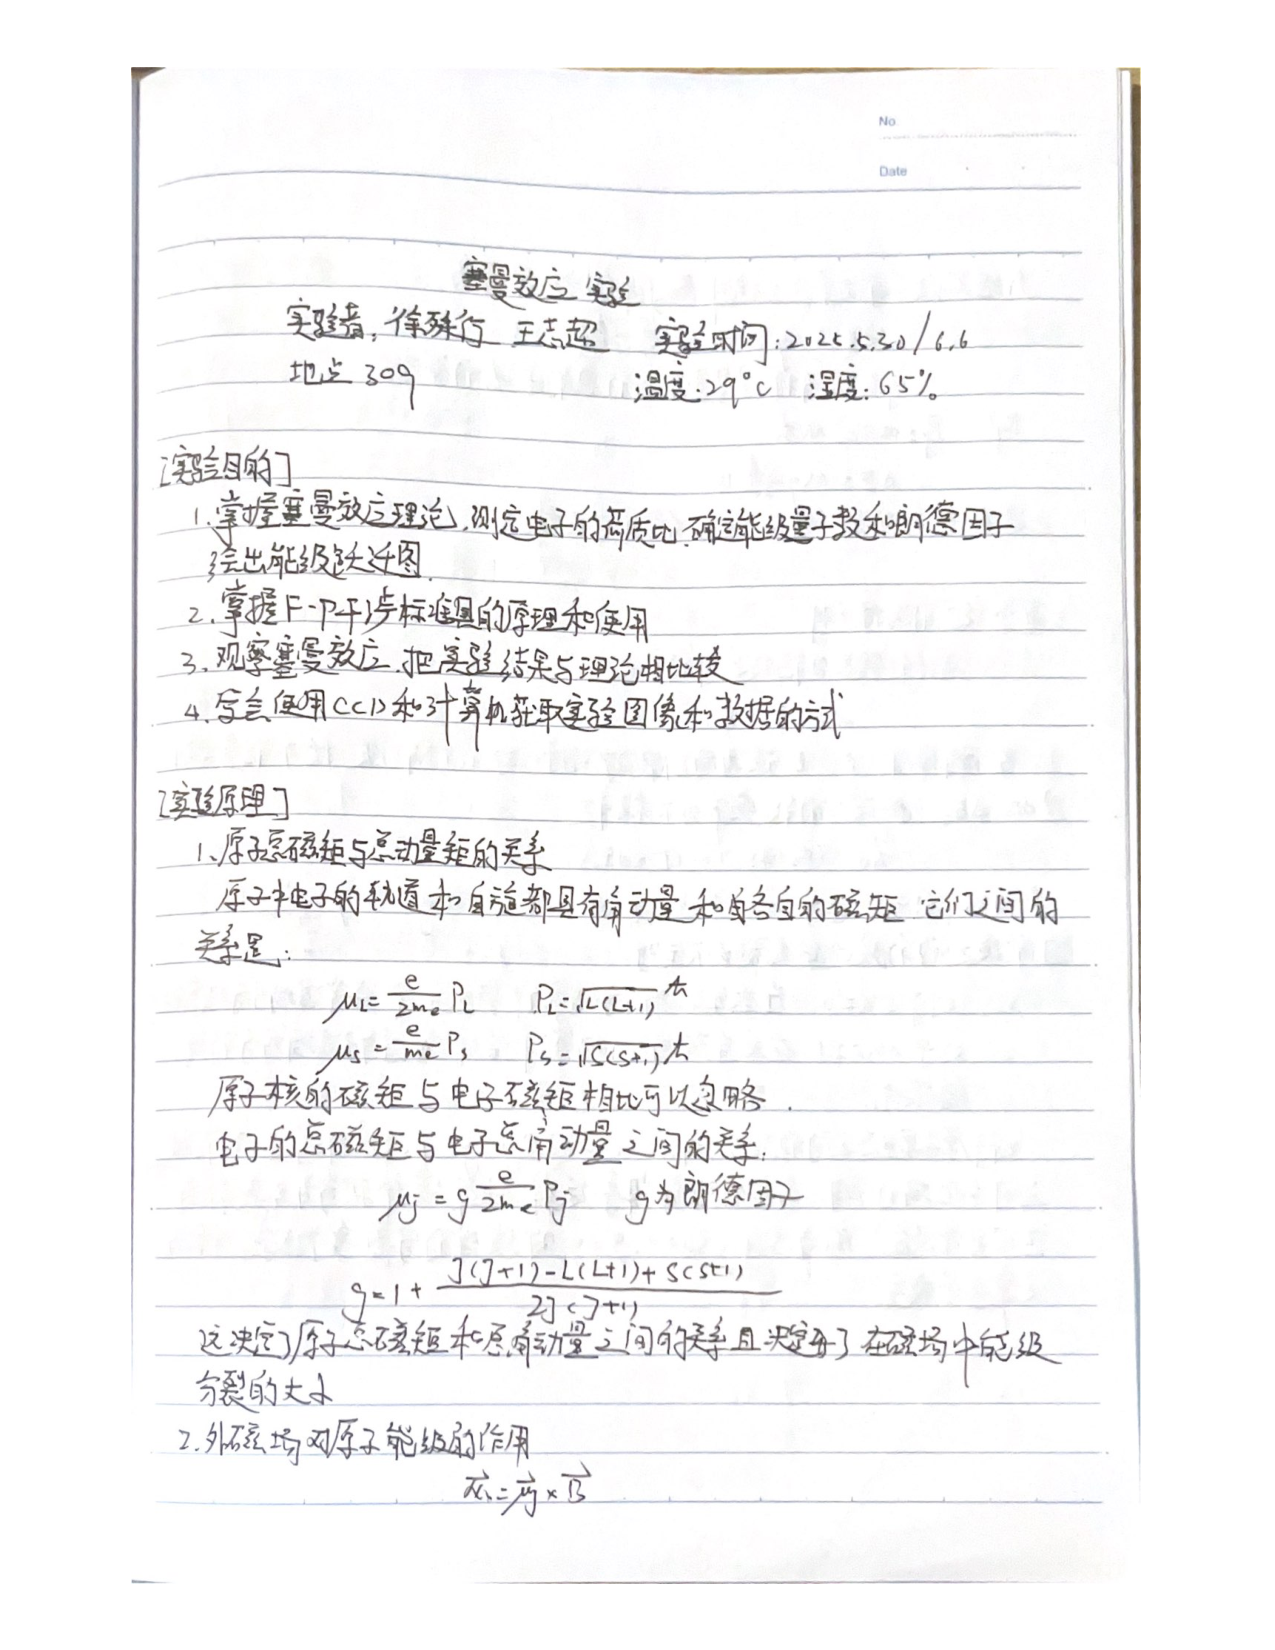
\includepdf[pages=-]{塞曼效应scan.pdf}

\end{document}